\documentclass[lang=cn,newtx,10pt,scheme=chinese]{elegantbook}
\usepackage[dvipsnames]{xcolor}
\usepackage{circuitikz}
\usepackage{annotate-equations}
\usepackage{minted}
\usetikzlibrary{tikzmark}
\usetikzlibrary{arrows.meta,
                bending,
                intersections,
                quotes,
                shapes.geometric}
\tcbuselibrary{minted,skins,breakable}
% 灵活版本（可选颜色）
\NewDocumentCommand{\mybox}{O{red} m m}{%
  \begin{tcolorbox}[colback=#1!5!white,colframe=#1!75!black,title=#2]
    #3
  \end{tcolorbox}%
}

\newtcolorbox{marker}[1][]{enhanced,
  before skip=2mm,after skip=3mm,
  boxrule=0.4pt,left=5mm,right=2mm,top=1mm,bottom=1mm,
  colback=yellow!50,
  colframe=yellow!20!black,
  sharp corners,rounded corners=southeast,arc is angular,arc=3mm,
  underlay={%
    \path[fill=tcbcolback!80!black] ([yshift=3mm]interior.south east)--++(-0.4,-0.1)--++(0.1,-0.2);
    \path[draw=tcbcolframe,shorten <=-0.05mm,shorten >=-0.05mm] ([yshift=3mm]interior.south east)--++(-0.4,-0.1)--++(0.1,-0.2);
    \path[fill=yellow!50!black,draw=none] (interior.south west) rectangle node[white]{\Huge\bfseries !} ([xshift=4mm]interior.north west);
    },
  drop fuzzy shadow,#1}

% ========== 通用代码盒子 ==========
\newtcblisting{codebox}[3][]{
  listing engine=minted,
  minted language=#2,
  listing only,
  colback=blue!5!white,
  colframe=blue!75!black,
  title=#3,
  fonttitle=\bfseries\sffamily,
  breakable,
  enhanced,
  drop shadow,
  sharp corners,
  boxrule=1pt,
  minted options={
    linenos,
    numbersep=3mm,
    breaklines,
    fontsize=\small,
    frame=lines,
    framesep=2mm,
    baselinestretch=1.2,
    escapeinside=ββ
  },
  #1
}



\newcommand{\py}[1]{%
  \colorbox{gray!10}{\mintinline{python}{#1}}%
}


\title{ElegantBook：优美的 \LaTeX{} 书籍模板}
\subtitle{Elegant\LaTeX{} 经典之作}

\author{Ethan Deng \& Liam Huang \& syvshc \& sikouhjw \& Osbert Wang}
\institute{Elegant\LaTeX{} Program}
\date{2022/12/31}
\version{4.5}
\bioinfo{自定义}{信息}

\extrainfo{注意：本模板自 2023 年 1 月 1 日开始，不再更新和维护！}

\setcounter{tocdepth}{3}

\logo{logo-blue.png}
\cover{cover.jpg}

% 本文档命令
\usepackage{array}
\newcommand{\ccr}[1]{\makecell{{\color{#1}\rule{1cm}{1cm}}}}

% 修改标题页的橙色带
\definecolor{customcolor}{RGB}{32,178,170}
\colorlet{coverlinecolor}{customcolor}
\usepackage{cprotect}

\addbibresource[location=local]{reference.bib} % 参考文献，不要删除

\begin{document}

\maketitle
\frontmatter

\tableofcontents

\mainmatter

\part{强化学习基础}

\chapter{强化学习简介}

\section{基本概念}

\textbf{强化学习}（reinforcement learning，RL）讨论的问题是智能体（agent）怎么在复杂、不确定的环境（environment）中最大化它能获得的奖励。

\begin{figure}[!ht]
\centering
\resizebox{1\textwidth}{!}{%
\begin{circuitikz}
\tikzstyle{every node}=[font=\LARGE]
\draw [ fill={rgb,255:red,214; green,141; blue,102} ] (23.75,21.5) rectangle  node {\LARGE 环境} (28,19.25);
\draw [ fill={rgb,255:red,150; green,166; blue,233} ] (23.75,28.25) rectangle  node {\LARGE 智能体} (28,26);
\draw [short] (32,26) -- (32,26);
\draw [short] (29.5,27.25) -- (29.5,27.25);
\draw [line width=1pt, short] (28,27.25) -- (30.75,27.25);
\draw [line width=1pt, ->, >=Stealth] (30.75,20.5) -- (28,20.5);
\draw [line width=1pt, ->, >=Stealth] (26,21.5) -- (26,26)node[pos=0.5, fill=white]{奖励$R_t$};
\draw [line width=1pt, dashed] (20.75,21.5) -- (20.75,19.25);
\draw [line width=1pt, short] (20.75,20.5) -- (16.75,20.5);
\draw [line width=1pt, short] (16.75,20.5) -- (16.75,27.25)node[pos=0.5, fill=white]{状态$S_t$};
\draw [line width=1pt, ->, >=Stealth] (16.75,27.25) -- (23.75,27.25);
\draw [line width=1pt, short] (30.75,27.25) -- (30.75,20.5)node[pos=0.5, fill=white]{动作$A_t$};
\draw [line width=1pt, ->, >=Stealth] (23.75,20.5) -- (20.75,20.5)node[pos=0.5, fill=white]{$S_{t+1}$};
\end{circuitikz}
}%
\caption{强化学习交互循环}
\label{fig:fig-rl-loop}
\end{figure}


\begin{itemize}
\item Agent：智能体，代理，智能代理
\item Environment：环境
\item State：状态
\item Reward：奖励
\item Action：动作，行动
\end{itemize}

强化学习由两部分组成：\textbf{智能体}和\textbf{环境}。在强化学习过程中，智能体与环境一直在交互。智能体在环境中获取某个状态后，它会利用该状态输出一个动作（action）。然后这个动作会在环境中被执行，环境会根据智能体采取的动作，输出下一个状态以及当前这个动作带来的奖励。智能体的目的就是尽可能多地从环境中获取奖励。

下面是一个倒立摆环境。

\begin{figure}[!ht]
\centering
\resizebox{1\textwidth}{!}{%
\begin{circuitikz}
\tikzstyle{every node}=[font=\LARGE]
\draw [ fill={rgb,255:red,0; green,0; blue,0} , line width=1pt ] (21.75,18) rectangle (25.75,16.25);
\draw [ color={rgb,255:red,60; green,58; blue,207} , fill={rgb,255:red,240; green,157; blue,112}, line width=1pt , rotate around={-25:(24.875, 20.25)}] (25,23) rectangle (24.75,17.5);
\draw [line width=1pt, short] (13.75,17.25) -- (33.5,17.25);
\draw [line width=1pt, ->, >=Stealth, dashed] (26,22.75) -- (31,26.75);
\draw [line width=1pt, ->, >=Stealth, dashed] (23.5,16.25) -- (19.5,12);
\node [font=\LARGE] at (31.75,27.25) {木杆};
\node [font=\LARGE] at (18.75,11.5) {推车};
\end{circuitikz}
}%
\caption{倒立摆环境}
\label{fig:fig-cartpole-env}
\end{figure}

在这个环境中，智能体是推车。

\begin{itemize}
\item 动作空间：推车有两个动作，\textbf{向左推}和\textbf{向右推}
\item 状态：
\begin{itemize}
	\item 推车的位置
	\item 推车的速度
	\item 杆子的角度
	\item 杆子的角速度
\end{itemize}

\item 奖励：推车采取向左推或者向右推的动作之后，只要杆子不倒下，奖励就是1。
\end{itemize}

游戏的结束条件：

\begin{itemize}
\item 推车将杆子推出了屏幕（失败）
\item 杆子倒下（失败）
\item 采取了200次推车的动作，杆子也没倒下（成功）
\end{itemize}

那么推车应该采取什么样的动作，杆子才能不倒下呢？或者说，推车应该采取什么样的\textbf{策略}（policy），杆子才能不倒下呢？因为只有杆子不倒下，我们才能不停的获得奖励。

如果推车每采取一个动作，杆子还能保持平衡，那么我们获得的\textbf{即时奖励}是1。

如果到游戏结束，杆子也没有倒下，那么我们将获得最大的奖励200。

而推车每次要采取什么动作，是取决于环境的状态的。也就是推车要根据环境的状态来决定下一步采取什么动作。例如：此时杆子向左偏，那么推车可能需要采取向左推的动作，才能使杆子不倒下。

换句话说，推车要采取的策略是一个\textbf{函数}。

\begin{figure}[!ht]
\centering
\resizebox{1\textwidth}{!}{%
\begin{circuitikz}
\tikzstyle{every node}=[font=\LARGE]
\node [font=\LARGE] at (19.5,21.5) {要采取的动作的概率分布   =   策略函数(环境的状态)};
\draw [ fill={rgb,255:red,215; green,29; blue,157} ] (35.5,24.25) rectangle (35.5,24);
\draw [ fill={rgb,255:red,215; green,29; blue,157} ] (19.25,24.75) rectangle (19.25,24.75);
\draw [ color={rgb,255:red,219; green,10; blue,10}, line width=1.2pt, short] (20.25,21) -- (22.5,21);
\draw [short] (12.5,12.5) -- (27.25,12.5);
\draw [ fill={rgb,255:red,165; green,216; blue,255} ] (15.5,15.25) rectangle (16.75,12.5);
\draw [ fill={rgb,255:red,178; green,242; blue,187} ] (21.5,19.75) rectangle (22.75,12.5);
\node [font=\LARGE] at (16.25,12) {向左推的概率0.3};
\node [font=\LARGE] at (22.25,12) {向右推的概率0.7};
\end{circuitikz}
}%
\caption{策略是一个函数}
\label{fig:fig-policy-function}
\end{figure}

而这里\textbf{要采取的动作}一般来说是一个概率分布。例如：向左推的概率=0.3，向右推的概率=0.7 。

然后从这个分布中进行采样，采样一个动作出来。当然也可以直接选概率最大的动作。

而我们使用什么样的策略呢？当然是能够让我们在游戏结束时，能够获得最大奖励的策略啦。

当然，这里选择策略有很多的讲究。如果我们每次采取的都是概率最大的动作，那么每次可能都会获得最大的即时奖励。如果这样做的话，可能到了一定的时候，不管向左推还是向右推获得的即时奖励可能都是0，也就是不管怎么推，杆子都会倒下（杆子偏离的角度太大，怎么推都没用）。也就是说，我们太看重眼前利益，忽略了长远的利益。这样就是只\textbf{利用}而不\textbf{探索}。所以有时也需要采取一下概率低的动作，探索一下环境，万一未来获得的奖励更多呢。

所以偶尔也需要采取一下概率小的动作。

\mybox[blue]{NOTE}{
    所谓\textbf{从概率分布中采样}的意思是，例如概率分布是向左推的概率是0.7，向右推的概率是0.3。那么从这个概率分布中采样一个动作出来，有70\%的概率采取的动作是向左推。但也有30\%的概率向右推。
}

举个例子：如果我们每次都去最熟悉的餐馆吃饭，可能体验都还可以。而如果去不熟悉的餐厅吃饭，可能体验不好，也可能体验超过了之前的餐馆。在舒适区只利用不探索，就会固步自封。冒险可能会受到伤害，但长期来看，可能会得到提升。

策略是智能体的动作模型，它决定了智能体的动作。它其实是一个函数，用于把输入的状态变成动作。

策略的数学符号是 $\pi$ ，所以策略也就是 $\pi$ 函数。即 $\pi(a | s)=p\left(a_{t}=a | s_{t}=s\right)$ 。输入一个状态 $s$ ，输出一个概率分布。用条件概率来看，就是在条件：状态为 $s$ 的情况下，策略采取动作 $a$ 的概率是多少。这个概率是智能体所有动作的概率，然后对这个概率分布进行采样，可得到智能体将采取的动作。比如可能是有 0.7 的概率往左，0.3 的概率往右，那么通过采样就可以得到智能体将采取的动作。

\bigskip
\bigskip
\bigskip
\begin{equation*}
    \pi(a|s) = p(
        \eqnmarkbox[NavyBlue]{p1}{a_t}=a|\eqnmarkbox[Lavender]{p2}{s_t}=s)
\end{equation*}
\annotate[yshift=1em]{above}{p1}{在状态为$s$时，采取动作$a$的概率}
\annotate[yshift=-1em]{below}{p2}{$t$时刻环境的状态为$s$}
\bigskip
\bigskip

所以有如下：

$$
\begin{aligned}
\pi(a=a_{_\text{向左推}}|s)=0.7 \\
\pi(a=a_{_\text{向右推}}|s)=0.3
\end{aligned}
$$

如果这个 $\pi$ 函数是一个神经网络，那么这就是\textbf{深度学习 + 强化学习 = 深度强化学习}。当今 AI 界最热门的话题。

所以玩倒立摆游戏的一个\textbf{回合}（episode）就是环境的状态为 $S_0$ ，推车采取动作 $A_0$ ，然后获得奖励 $R_0$ ，然后环境的状态转移到了 $S_1$ ，推车接着采取动作 $A_1$ ，然后获得奖励 $R_1$ ...。下标是时刻，或者时间步。把它们写到一起，就是一个\textbf{轨迹}（trajectory）。轨迹用数学符号 $\tau$ 表示，读作\textbf{掏}。

$$
\tau = (S_0,A_0,R_0,S_1,A_1,R_1,S_2,A_2,R_2\dots)
$$

由于根据环境的状态，采取的动作是从一个概率分布中采样得到的，所以轨迹会有很多很多条。

\begin{figure}[!ht]
\centering
\resizebox{1\textwidth}{!}{%
\begin{circuitikz}
\tikzstyle{every node}=[font=\LARGE]
\draw [ fill={rgb,255:red,219; green,20; blue,20} ] (9.75,21.25) circle (0.5cm);
\draw [short] (10.25,21.25) -- (15.5,21.25)node[pos=0.5, fill=white]{向左推};
\draw [ fill={rgb,255:red,219; green,20; blue,20} ] (16,21.25) circle (0.5cm);
\draw [short] (16.5,21.25) -- (21.75,21.25)node[pos=0.5, fill=white]{向左推};
\draw [ fill={rgb,255:red,219; green,20; blue,20} ] (22.25,21.25) circle (0.5cm);
\draw [short] (22.5,21.25) -- (27.75,21.25)node[pos=0.5, fill=white]{向左推};
\draw [ fill={rgb,255:red,219; green,20; blue,20} ] (28.25,21.25) circle (0.5cm);
\draw [short] (28.5,21.25) -- (33.75,21.25)node[pos=0.5, fill=white]{向左推};
\draw [ fill={rgb,255:red,219; green,20; blue,20} ] (34.25,21.25) circle (0.5cm);
\draw [->, >=Stealth] (34.75,21.25) -- (37.25,21.25);
\node [font=\LARGE, color={rgb,255:red,186; green,18; blue,18}] at (39.25,21.25) {游戏失败};
\draw [ fill={rgb,255:red,219; green,20; blue,20} ] (9.75,17.75) circle (0.5cm);
\draw [short] (10.25,17.75) -- (15.5,17.75)node[pos=0.5, fill=white]{向右推};
\draw [ fill={rgb,255:red,219; green,20; blue,20} ] (16,17.75) circle (0.5cm);
\draw [short] (16.5,17.75) -- (21.75,17.75)node[pos=0.5, fill=white]{向右推};
\draw [ fill={rgb,255:red,219; green,20; blue,20} ] (22.25,17.75) circle (0.5cm);
\draw [short] (22.5,17.75) -- (27.75,17.75)node[pos=0.5, fill=white]{向右推};
\draw [ fill={rgb,255:red,219; green,20; blue,20} ] (28.25,17.75) circle (0.5cm);
\draw [short] (28.5,17.75) -- (33.75,17.75)node[pos=0.5, fill=white]{向右推};
\draw [ fill={rgb,255:red,219; green,20; blue,20} ] (34.25,17.75) circle (0.5cm);
\draw [->, >=Stealth] (34.75,17.75) -- (37.25,17.75);
\node [font=\LARGE, color={rgb,255:red,186; green,18; blue,18}] at (39.25,17.75) {游戏失败};
\draw [ fill={rgb,255:red,219; green,20; blue,20} ] (9.75,14.25) circle (0.5cm);
\draw [short] (10.25,14.25) -- (15.5,14.25)node[pos=0.5, fill=white]{向左推};
\draw [ fill={rgb,255:red,219; green,20; blue,20} ] (16,14.25) circle (0.5cm);
\draw [short] (16.5,14.25) -- (21.75,14.25)node[pos=0.5, fill=white]{向右推};
\draw [ fill={rgb,255:red,219; green,20; blue,20} ] (22.25,14.25) circle (0.5cm);
\draw [short] (22.5,14.25) -- (27.75,14.25)node[pos=0.5, fill=white]{向左推};
\draw [ fill={rgb,255:red,219; green,20; blue,20} ] (28.25,14.25) circle (0.5cm);
\draw [short] (28.5,14.25) -- (33.75,14.25)node[pos=0.5, fill=white]{向右推};
\draw [ fill={rgb,255:red,219; green,20; blue,20} ] (34.25,14.25) circle (0.5cm);
\draw [->, >=Stealth] (34.75,14.25) -- (37.25,14.25);
\node [font=\LARGE, color={rgb,255:red,18; green,186; blue,91}] at (39.25,14.25) {游戏成功};
\node [font=\LARGE] at (21.75,12.25) {$\begin{array}{c}
    \vdots \\ \vdots
\end{array}$};
\end{circuitikz}
}%
\caption{无数条轨迹}
\label{fig:fig-trajectory-example}
\end{figure}

\section{价值函数（Value Function）}

当位于时刻 $t$ 时，环境此时处于状态 $S_t$ ，然后我们根据策略函数开始采取动作，那么未来我们一共能获得多少奖励呢？环境处于状态 $S_t$ ，我们采取的动作是 $A_t$ ，获取的奖励是 $R_t$ ，然后环境的状态从 $S_t$ 转移到了 $S_{t+1}$ ，然后采取动作 $A_{t+1}$ ，然后获得即时奖励 $R_{t+1}$ ，然后环境的状态从 $S_{t+1}$ 转移到了 $S_{t+2}$ ，然后环境会给我们即时奖励 $R_{t+2}$ ，......。

但是未来的奖励不如现在的奖励有吸引力，所以需要\textbf{打折}。那么，从 $t$ 时刻起，未来一共获得的奖励叫做\textbf{回报}（或者收益，Return）。

$$
G_t = R_t + \gamma R_{t+1} + \gamma^2 R_{t+2} + \cdots
$$

$\gamma$ 叫做折扣因子。随着时间的推移，奖励会被 $\gamma$ 指数级削弱。这个 $\gamma$ 被称为折扣因子（discount rate），其被设定为 $0.0$ 和 $1.0$ 之间的实数。如果折扣因子是 $0.9$，那么有以下式子成立。

$$
G_t = R_t + 0.9 R_{t+1} + 0.81 R_{t+2} + \cdots
$$

引入折现率主要是为了防止连续性任务的收益变得无穷大。在连续性任务中，如果没有折扣因子（或 $\gamma=1$ ），那么收益就会发散到无穷大。因此，设置折扣因子可以防止收益的发散。

折扣因子也使近期的奖励显得更加重要。这解释了人类乃至生物的许多行动原理。例如，你会选择今天拿到 10000 元还是一年后拿到 20000 元？如果折扣因子使未来的回报呈指数级下降，那么眼前的回报就会更有吸引力。

如果我们用倒立摆作为例子，然后我们运行两个时间步。得到下图。

\begin{figure}[!ht]
\centering
\resizebox{1\textwidth}{!}{%
\begin{circuitikz}
\tikzstyle{every node}=[font=\normalsize]
\draw  (7.25,18.5) circle (1cm) node {\LARGE 起点} ;
\draw  (14,21.5) circle (1cm) node {\LARGE 状态$1$} ;
\draw  (14,15) circle (1cm) node {\LARGE 状态$1'$} ;
\draw  (25.25,24) circle (1cm) node {\LARGE 状态$2$} ;
\draw  (25.25,20.25) circle (1cm) node {\LARGE 状态$2'$} ;
\draw  (25.25,16) circle (1cm) node {\LARGE 状态$2''$} ;
\draw  (25.25,12) circle (1cm) node {\LARGE 状态$2'''$} ;
\draw [->, >=Stealth] (8,19) -- (13.25,21)node[pos=0.5, fill=white]{向左推0.7};
\draw [->, >=Stealth] (8.25,18.25) -- (13,15.5)node[pos=0.5, fill=white]{向右推0.3};
\draw [->, >=Stealth] (15,22) -- (24.25,23.75)node[pos=0.5, fill=white]{向右推0.5};
\draw [->, >=Stealth] (15,21) -- (24.5,19.75)node[pos=0.5, fill=white]{向左推0.5};
\draw [->, >=Stealth] (15,15.5) -- (24,16.25)node[pos=0.5, fill=white]{向左推0.2};
\draw [->, >=Stealth] (14.75,14.25) -- (24,12.25)node[pos=0.5, fill=white]{向右推0.8};
\end{circuitikz}
}%
\caption{倒立摆环境运行2个时间步}
\label{fig:fig-two-timesteps}
\end{figure}

可以看到，一共有 4 条轨迹。每条轨迹都有一个总的回报。而每条轨迹也都有一个产生的概率。那么我们如何评估在环境处于状态 $S_t$ 时，一直采取策略 $\pi$ 未来会获得多少回报呢？也就是未来的预期回报（回报的期望值）是多少呢？那就是\textbf{状态价值函数}（State Value Function）。

$$
V_{\pi}(s) = \mathbb{E}_{\pi}\left[G_{t} \mid S_{t}=s\right]=\mathbb{E}_{\pi}\left[\sum_{k=0}^{\infty} \gamma^{k} R_{t+k} \mid S_{t}=s\right], \text{对于所有的} s \in S
$$

\mybox[blue]{NOTE}{
    状态价值函数，衡量的是在环境处于状态 $s$ 时，一直按照策略 $\pi$ 来采取动作，最终的预期回报。
}

状态价值函数的另一种重要的表示形式。

$$
\begin{aligned}
V_\pi(S_t=s)
&= \mathbb{E}_\pi[R_t+\gamma V_\pi(S_{t+1}=s')|S_t=s] \\
\end{aligned}
$$

哈哈。

\mybox[blue]{NOTE：贝尔曼期望方程}{
$$
\begin{aligned}
V_\pi(S_t)
&= \mathbb{E}_\pi[R_t+\gamma V_\pi(S_{t+1})|S_t] \\
\end{aligned}
$$
}

直观解释：

当前环境对你的价值 = 当前环境现在给你的奖励 + 折扣因子 $\times$ 未来环境对你的价值

你对公司的评估 = 现在公司给你的薪资 + 折扣因子 $\times$ 你对公司未来的评估

也就是你觉得现在公司怎么样？得看公司现在给你开的钱和你觉得公司未来的前景，综合考虑。

现在给的钱少，但是你觉得公司前景不错（折扣因子0.99），那么你对公司的评估也不错。

现在给的钱很多，但是你觉得公司前景会倒闭（折扣因子0.01，但如果不倒闭公司未来前景家这也很不错，但是倒闭的概率很大），那么你对公司的评估也不错。

还有一种可能，现在钱很少，公司倒闭的可能性很大，但一旦公司每倒闭，就很牛逼。

\section{倒立摆环境编程实践}

\begin{codebox}{bash}{安装倒立摆环境}
$ pip install gym==0.25.2
$ pip install numpy==1.26
$ pip install pygame
\end{codebox}

然后我们来创建一个倒立摆环境

\begin{codebox}{python}{创建倒立摆环境}
import gym
# 创建倒立摆环境
env = gym.make('CartPole-v0')
\end{codebox}

这样就生成了倒立摆的环境，见图\ref{fig:fig-cartpole-env}。

将推车向右或向左移动，以保持杆子的平衡。倒立摆的结束条件是杆子的平衡被打破（杆子超过一定的角度），或者推车的移动位置超出了某个范围。

下面继续执行以下代码。

\begin{codebox}{python}{}
state = env.reset() # 重置环境的状态
print(state) # 初始状态
action_space = env.action_space # 推车有几个动作？（向左推，向右推）
print(action_space) # 行动的维度
\end{codebox}

上面的代码通过 \py{state = env.reset()} 获得了初始状态。观察它的输出，你会发现它是拥有 4 个元素的数组。作为参考，下面依次列出这 4 个元素。

\begin{itemize}
\item 推车的位置
\item 推车的速度
\item 杆子的角度
\item 杆子的角速度
\end{itemize}

另外，我们可以通过 \py{env.action_space} 获得行动的维度（可采取的行动数）。它的输出是一个名为 \py{Discrete(2)} 的类实例。这意味着有两个候选行动。具体来说，0 对应的是向左移动推车的行动，1 对应的是向右移动推车的行动。下面实际地采取行动，向前推进一个时间步。

\begin{codebox}{python}{}
action = 0 # 或者 1
next_state, reward, done, info = env.step(action)
print(next_state)
\end{codebox}

上面的代码通过 \py{env.step(action)} 采取行动。作为结果 ，我们得到了以下 4 个信息。

\begin{itemize}
\item 下一个状态\py{next_state}
\item 奖励\py{reward}
\item 是否结束的标志位\py{done}
\item 附加信息\py{info}
\end{itemize}

\py{reward}是标量值（\py{float}）。这次的任务在保持平衡的时候总是会得到奖励1。\py{info}包含有助于调试的信息（如环境模型）。但在实现和评估强化学习的算法时，基本不会用到\py{info}。

我们先来实现一个随机智能体。也就是这个智能体的策略非常简单，无论环境处于什么状态，我们都是从两个动作中随机采样一个动作。

\begin{codebox}{python}{随机策略}
import numpy as np
import gym
import time

env = gym.make('CartPole-v0')
state = env.reset()
done = False
action_desc = {0: "向左推", 1: "向右推"}
total_reward = 0.0
reward_list = []
gamma = 0.99

while not done:
    env.render()β\tikzmark{randompolicy1}β
    action = np.random.choice([0, 1])β\tikzmark{randompolicy2}β
    next_state, reward, done, info = env.step(action)β\tikzmark{randompolicy3}β
    print(f"采取动作： \
           {action_desc.get(action, '未知动作')}，\
           获得奖励：{reward}，\
           转移到下一个状态：{next_state}")
    reward_list.append(reward)
    time.sleep(0.1)

for r in reward_list[::-1]:β\tikzmark{randompolicy4}β
    total_reward = r + gamma * total_reward

print('回报（收益）：', total_reward)
env.close()
\end{codebox}

\begin{tikzpicture}[
  remember picture,
  overlay,
  annotation/.style={
    inner sep=0pt,
    outer sep=0pt,
    outer xsep=1mm,
    fill=yellow!80!black,
    text width=4cm
  },
  >={Stealth[inset=0pt, angle=45:7pt]}
]
\draw[<-] (pic cs:randompolicy1)  ++(0.5,0.4) -| ++(2,1.5)
node[annotation, below right]
{渲染倒立摆环境};
\draw[<-] (pic cs:randompolicy2)  ++(0.5,0.4) -| ++(2,1.5)
node[annotation, below right]
{随机选择一个动作};
\draw[<-] (pic cs:randompolicy3)  ++(0.5,0.4) -| ++(2,1.5)
node[annotation, below right]
{采取动作，返回
\begin{itemize}
    \item 环境的下一个状态next\_state
    \item 即时奖励reward
    \item 是否结束done
    \item 调试信息info
\end{itemize}
};
\draw[<-] (pic cs:randompolicy4)  ++(0.5,0.4) -| ++(2,1.5)
node[annotation, below right]
{逆序计算$G_t = R_t + \gamma G_{t+1}$};
\end{tikzpicture}


\mybox[blue]{回报（总奖励的逆序计算）}{
从时间 0 开始的回报为
$G_0 = R_0 + \gamma R_1 + \gamma^2R_2 + \gamma^3R_3 = R_0 + \gamma G_1$
\\
从时间 1 开始的回报为
$G_1 = R_1 + \gamma R_2 + \gamma^2R_3 = R_1 + \gamma G_2$
\\
从时间 2 开始的回报为
$G_2 = R_2 + \gamma R_3 = R_2 + \gamma G_3$
\\
从时间 3 开始的回报为
$G_3 = R_3$
\\
所以
$G_t = R_t + \gamma G_{t+1}$
\\
所以我们要进行逆序计算。
\mybox[red]{霍纳法则（秦九韶算法）}{
$$
\begin{aligned}
& a_0 + a_1x + a_2x^2 + \cdots + a_nx^n \\
= & a_0 + x \left(a_1 + x\left(a_2 + x\left(a_3+\cdots+x\left(a_{n-1}+xa_n\right)\cdots\right)\right)\right)
\end{aligned}
$$
}
\mybox[pink]{动态规划思想}{
前向过程：采样一条轨迹，得到每个时刻的即时奖励。
\\
反向过程：逆序计算回报。
}
}

由于我们使用的是\textbf{随机策略}，所以倒立摆游戏很快就结束了。

\section{马尔可夫决策过程}

\subsection{基本概念}

马尔可夫决策过程（MDP，Markov Decision Process）。决策过程是智能体通过与环境互动决定其行动的过程。

智能体所处的环境根据其行动而发生改变。在强化学习中，这种情况被称为环境的“状态”（state）。在MDP中，状态的变化取决于智能体的行动，智能体在环境的状态迁移后执行新的行动。

在MDP中，我们需要“时间”的概念。在某一时刻，智能体会采取行动并因此迁移到一个新的状态。此时的时间单位叫作“时间步”。由于时间步是智能体做出决定的间隔时间，因此它的实际单位取决于问题。

智能体要考虑的是将来获得的奖励总和，而不是眼前的奖励。换句话说，智能体的目标是实现奖励总和最大化。

在MDP中，智能体与环境之间会进行互动。要点在于当智能体采取行动时，状态会发生迁移，随之获得的奖励也会相应改变。

参见图\ref{fig:fig-rl-loop}。

假设在时刻 $t$ 的状态是 $S_t$ 。基于这个状态 $S_t$ ，智能体执行行动 $A_t$ ，获得奖励 $R_t$ 并迁移到下一个状态 $S_{t+1}$ 。智能体与环境之间的这种实际的互动产生了以下迁移。

$$
S_0,A_0,R_0,S_1,A_1,R_1,S_2,A_2,R_2,\cdots
$$

这个时间序列数据从第一个状态 $S_0$ 开始。在状态 $S_0$ ，智能体执行行动 $A_0$ 并获得奖励 $R_0$ 。时刻变为 $1$ ，状态变为 $S_1$ 。接下来，基于状态 $S_1$ ，智能体执行行动 $A_1$ 并获得奖励 $R_1$，然后进入下一个状态 $S_2\cdots\cdots$ 这个流程不断持续下去。

MDP通过数学式来表示智能体、环境以及二者之间的互动。要做到这一点，需要用数学式来表达以下 3 个要素。

\begin{itemize}
\item 状态迁移：状态如何迁移。
\item 奖励：如何给予奖励。
\item 策略：智能体如何决定行动。
\end{itemize}

\subsection{状态转移}

假设智能体现在处于状态 $s$ 并执行了行动 $a$ ，那么转移到下一个状态 $s'$ 的概率可以用如下方式表示。

$$
p(s'|s,a)
$$

\mybox[blue]{状态和观察}{
状态（state）：如果能观察到整个环境完整的信息，就叫做状态
\\
观察（observation）：只能观察到环境的部分状态（信息）
}

竖杠 $\vert$ 的右侧是表示“条件”的概率变量。对于当前问题，条件对应于在状态 $s$ 选择了行动 $a$ 。在给定这两个条件的情况下，转移到 $s'$ 的概率可以表示为 $p(s'|s,a)$ 。像 $p(s'|s,a)$ 这样的概率叫作状态迁移概率（state transition probability）。

$p(s'|s,a)$ 决定了下一个状态 $s'$ 只取决于当前状态 $s$ 和行动 $a$ 。

换句话说，状态转移不需要过去的信息——此前处于什么状态以及执行了哪些行动。这个特性被称为\textbf{马尔可夫性质}（Markov property）。

MDP通过假设马尔可夫性质的存在来模拟状态转移和奖励。引入马尔可夫性质主要是为了使问题更容易解决。如果不假定马尔可夫性质，那么就必须考虑之前的所有状态和行动，而且组合的数量会呈指数级增长。

\subsection{奖励函数}

当智能体处于状态 $s$ ，执行行动 $a$，下一个状态是 $s'$ 时，得到的奖励由函数 $r(s,a,s')$ 定义。$r(s,a,s')$ 叫做\textbf{奖励函数}。

\mybox[blue]{倒立摆环境中的奖励}{
倒立摆环境中的奖励是确定性的，只要木杆不倒下，就给奖励 1 。
\\
而通常情况下，奖励函数也是一个神经网络。
}

\subsection{策略}

策略表示智能体如何决定其行动。策略的关键在于它使得智能体仅根据当前状态来决定其行动。之所以说只基于当前状态就足够了，是因为环境的迁移是符合马尔可夫性质的。

环境的状态迁移只以当前状态 $s$ 和行动 $a$ 为条件来决定下一个状态 $s'$ ，而不需要先前的信息。同样，奖励也是基于当前状态 $s$ 、行动 $a$ 和迁移后的状态 $s'$ 来决定的。这意味着关于环境的所有必要信息都在当前状态中。因此，智能体只需基于当前状态即可决定其行动。

\mybox[blue]{NOTE}{
MDP的马尔可夫性质可以被看作是对环境而不是对智能体的约束。这意味着为了满足马尔可夫性质，环境需要保持某个“状态”。从智能体的角度来看，在当前状态下有足够的信息来做出最佳选择，所以它可以在此基础上采取行动。
}

智能体的行动是由随机性策略决定的，数学式如下所示。

$$
\pi(a|s)
$$

$\pi(a|s)$ 表示在状态 $s$ 下采取行动 $a$ 的概率。

我们已经成功地用数学式来表示状态迁移、奖励函数和策略。接下来让我们使用这三者来定义MDP的目标。

\subsection{MDP的目标}

到目前为止，我们已经用数学式描述了环境和智能体的行动。简要回顾一下，智能体根据策略 $\pi(a|s)$ 采取行动。首先，它根据它的行动和状态迁移概率 $p(s'|s,a)$ 迁移到下一个状态。然后，它根据奖励函数 $r(s,a,s')$ 获得奖励。在这个框架内，MDP的目标是找到\textbf{最优策略}（optimal policy）。最优策略是使收益最大化的策略。

\subsection{收益}

为了定义收益，我们思考这样一个场景：设时刻为 $t$ ，状态为 $S_t$ （其中 $t$ 是任意值）。然后，智能体根据策略 $\pi$ 执行行动 $A_t$ ，获得奖励 $R_t$ ，之后迁移到新状态 $S_{t+1}$，这个过程不断重复进行。在这种情况下，收益 $G_t$ 的定义如下所示。

$$
G_t = R_t + \gamma R_{t+1} + \gamma^2 R_{t+2} + \cdots
$$

$\gamma$ 为折扣因子。

\subsection{状态价值函数}

我们已经重新定义了“收益”。智能体的目标是使这种收益最大化。这里有一点需要注意，那就是智能体和环境的行动可能是“随机性”的。智能体可能随机地决定行动，状态也可能随机迁移。在这种情况下，获得的收益将呈现随机的特点。即使从相同的状态开始，不同回合的收益也随机变化。例如，某个回合的收益为 $10.4$ ，另一个回合的收益为 $8.7$ 。

为了处理这种随机行动，需要使用期望值或“收益的期望值”作为衡量标准。收益的期望值的数学式如下所示。

$$
v_\pi(s) = \mathbb{E}[G_t|S_t=s,\pi]
$$

我们指定的条件是状态 $S_t$ 为 $s$ 智能体的策略为 $\pi$ （其中时刻 $t$ 是任意值）。在这些条件下，智能体获得的收益的期望值为上面的公式。在这里，我们用特殊符号 $v_\pi(s)$ 来表示收益的期望值。就是\textbf{状态价值函数}（state-value function）。

在公式的右侧，智能体的策略 $\pi$ 被作为条件给出。这是因为如果策略 $\pi$ 发生变化，那么智能体获得的奖励也会发生变化，而这些奖励的总和，即收益也会发生变化。为了明确这一点，状态价值函数通常会写作 $v_\pi(s)$ ，将 $\pi$ 写在 $v$ 的右下角。此外，上面的公式也可以写成下面的形式。

$$
v_\pi(s) = \mathbb{E}_\pi[G_t|S_t=s]
$$

在上面的式子中，记载 $\pi$ 的位置是 $\mathbb{E}_\pi$ 。与式（1）一样，这么写的含义是策略 $\pi$ 是作为条件给出的。从现在起，本教程将采取式（2）的风格来书写式子。

在强化学习中，我们的目标是获得最优策略。

最优策略的状态价值函数叫作\textbf{最优状态价值函数}（optimal state-value function）。可以使用 $v_*$ 来表示最优状态价值函数。

\section{贝尔曼方程}

贝尔曼方程是在MDP中成立的最重要的方程，为许多强化学习算法提供了重要基础。

这里使用骰子作为例子。我们使用的骰子是理想的六面体，每一面的数字出现的概率都是 $\frac{1}{6}$ 。在数学式中，我们用随机变量 $x$ 表示掷骰子出现的数字， $x$ 是 $1$ 和 $6$ 之间的整数。那么每个数字出现的概率就是 $\frac{1}{6}$ 。 我们用 $p(x)=\frac{1}{6}$ 表示骰子的数字出现的概率。现在来计算掷骰子的期望值。计算式如下所示。

$$
\begin{aligned}
\mathbb{E}[x] &= 1\times\frac{1}{6}+2\times\frac{1}{6}+3\times\frac{1}{6}+4\times\frac{1}{6}+5\times\frac{1}{6}+6\times\frac{1}{6} \\
&= 3.5
\end{aligned}
$$

如上所述，期望值是在所有情况下“出现的数字”和“概率”相乘并加在一起得到的和。顺带一提，如果使用 $\sum$ 符号，那么期望值的数学式如下所示。

$$
\mathbb{E}[x]=\sum_xxp(x)
$$

另外， $x$ 和 $y$ 同时发生的概率（这叫作“联合概率”）如下所示。

$$
p(x,y)=p(x)p(y|x)=p(y)p(x|y)
$$

假设奖励用 $r(x,y)$ 来表示，那么奖励的期望值如下

$$
\begin{aligned}
\mathbb{E}[r(x,y)] &= \sum_x\sum_yp(x,y)r(x,y) \\
&= \sum_x\sum_yp(x)p(y|x)r(x,y)
\end{aligned}
$$

回顾收益（回报）的定义。

$$
G_t = R_t + \gamma R_{t+1} + \gamma^2 R_{t+2} + \cdots
$$

那么有以下公式

$$
G_{t+1} = R_{t+1} + \gamma R_{t+2} + \gamma^2 R_{t+3} + \cdots
$$

所以有以下递推公式：

$$
\begin{aligned}
G_t &= R_t+\gamma R_{t+1}+\gamma^2R_{t+2}+\cdots \\
&= R_t + \gamma(R_{t+1}+\gamma R_{t+2}+\cdots) \\
&= R_t+\gamma G_{t+1}
\end{aligned}
$$

这种递推关系被用于强化学习的许多理论和算法中。

下面将递推公式代入状态价值函数的定义式中。状态价值函数是收益的期望值，其数学式的定义如下所示。

$$
v_\pi(s) = \mathbb{E}_\pi[G_t|S_t=s]
$$

如上面的公式所示，状态 $s$ 的价值函数被表示为 $v_\pi(s)$ 。将递推公式带入上面的式子的 $G_t$ 中，得到下面的式子：

$$
\begin{aligned}
v_\pi(s) &= \mathbb{E}_\pi[G_t|S_t=s] \\
&= \mathbb{E}_\pi[R_t+\gamma G_{t+1}|S_t=s] \\
&= \mathbb{E}_\pi[R_t|S_t=s] + \gamma\mathbb{E}_\pi[G_{t+1}|S_t=s]
\end{aligned}
$$

\mybox[blue]{期望的线性性质}{
$$
\mathbb{E}[X+Y] = \mathbb{E}[X] + \mathbb{E}[Y]
$$
}

先来推导上面公式中的第一项 $\mathbb{E}_\pi[R_t|S_t=s]$ 。

$\mathbb{E}_\pi[R_t|S_t=s]$ 的含义是在 $t$ 时刻，环境的状态是 $s$ ，那么从 $t$ 时刻开始，获得的回报的期望是多少呢？那么需要考虑所有的情况，然后加起来就可以了。

$$
\mathbb{E}_\pi[R_t|S_t=s]=\sum_a\sum_{s'}\pi(a|s)p(s'|s,a)r(s,a,s')
$$

如上面的数学式所示，将智能体行动的概率 $\pi(a|s)$ 、要迁移的状态的概率 $p(s'|s,a)$ 和奖励函数 $r(s,a,s')$ 相乘。对所有候选项都进行上述计算，得到它们的总和。

第一项推导完毕，接下来推导第二项。

\bigskip
\bigskip
\bigskip
\begin{equation*}
    v_\pi(s)=\eqnmarkbox[NavyBlue]{bellman1}{\mathbb{E}_\pi[R_t|S_t=s]}+\eqnmarkbox[Lavender]{bellman2}{\gamma\mathbb{E}_\pi[G_{t+1}|S_t=s]}
\end{equation*}
\annotate[yshift=1em]{above}{bellman1}{$\sum_{a,s'}\pi(a|s)p(s'|s,a)r(s,a,s')$}
\annotate[yshift=-1em]{below}{bellman2}{接下来推导这一项}
\bigskip
\bigskip

剩下的项是 $\gamma\mathbb{E}_\pi[G_{t+1}|S_t=s]$ 。由于 $\gamma$ 是常数，因此我们要看的是 $\mathbb{E}_\pi[G_{t+1}|S_t=s]$ 。这个式子虽然与状态价值函数的定义式相似，但在 $G_{t+1}$ 的部分有所不同。状态价值函数的式子如下所示，式子中是 $G_t$ ，而不是 $G_{t+1}$ 。

$$
v_\pi(s) = \mathbb{E}_\pi[G_t|S_t=s]
$$

因此，我们首先要将 $t+1$ 代入上面的式子的 $t$ 中。式子变化如下。

$$
v_\pi(s) = \mathbb{E}_\pi[G_{t+1}|S_{t+1}=s]
$$

这就是状态 $S_{t+1}=s$ 时的价值函数。接下来要关注的是 $\mathbb{E}_\pi[G_{t+1}|S_t=s]$ 。这是在当前时刻为 $t$ 时，下一个时刻 $(t+1)$ 的收益期望值。解决的关键在于将条件 $S_t=s$ 变为 $S_{t+1}=s$ 的形式。换句话说，就是要进入下一个时刻。

通过观察可以得到

$$
\begin{aligned}
\mathbb{E}_\pi[G_{t+1}|S_t=s] &= \sum_{a,s'}\pi(a|s)p(s'|s,a)\mathbb{E}_\pi[G_{t+1}|S_{t+1}=s'] \\
&= \sum_{a,s'}\pi(a|s)p(s'|s,a)v_\pi(s')
\end{aligned}
$$

完成第二项的展开以后，汇总一下得到

$$
\boxed{
\begin{aligned}
v_\pi(s) &= \mathbb{E}_\pi[R_t|S_t=s] + \gamma\mathbb{E}_\pi[G_{t+1}|S_t=s] \\
&= \sum_{a,s'}\pi(a|s)p(s'|s,a)r(s,a,s')+\gamma\sum_{a,s'}\pi(a|s)p(s'|s,a)v_\pi(s') \\
&= \sum_{a,s'}\pi(a|s)p(s'|s,a)\{r(s,a,s')+\gamma v_\pi(s')\}
\end{aligned}
}
$$

上面的式子就是大名鼎鼎的\textbf{贝尔曼方程}。贝尔曼方程是表示状态 $s$ 的价值函数和下一个可能的状态 $s'$ 的价值函数之间关系的式子。这个贝尔曼方程对所有状态 $s$ 和所有策略 $\pi$ 都成立。

状态价值函数的贝尔曼方程的另一种重要的表示形式：\textbf{贝尔曼期望方程}。

$$
\boxed{
\begin{aligned}
V_\pi(S_t)
&= \mathbb{E}_\pi[R_t+\gamma V_\pi(S_{t+1})|S_t] \\
\end{aligned}
}
$$

\mybox[blue]{贝尔曼期望方程的推导过程}{
$$
\begin{aligned}
V_\pi(S_t) &= \mathbb{E}_\pi[G_t|S_t] \\
&= \mathbb{E}_\pi\left[\sum_{k=0}^\infty\gamma^kR_{t+k}\mid S_t\right] \\
&= \mathbb{E}_\pi\left[R_t+\gamma\sum_{k=0}^\infty\gamma^kR_{t+k+1}\mid S_t\right] \\
&= \mathbb{E}_\pi[R_t+\gamma G_{t+1}|S_t] \\
&= \mathbb{E}_\pi[R_t|S_t]+\gamma \mathbb{E}_\pi[G_{t+1}|S_t] \\
&= \mathbb{E}_\pi[R_t|S_t]+\gamma \mathbb{E}_\pi[\mathbb{E}_\pi [G_{t+1}|S_{t+1}]|S_t] \\
&= \mathbb{E}_\pi[R_t|S_t]+\gamma \mathbb{E}_\pi[V_\pi(S_{t+1})|S_t] \\
&= \mathbb{E}_\pi[R_t+\gamma V_\pi(S_{t+1})|S_t] \\
\end{aligned}
$$
\mybox[red]{全期望公式}{
全期望公式：$\mathbb{E}[X]=\mathbb{E}[\mathbb{E}[X|Y]]$
\\
条件期望的迭代公式：$\mathbb{E}[X|Y]=\mathbb{E}[\mathbb{E}[X|Z]|Y]$
}
}

\section{下一步}

智能体的目标是使收益最大化。这里有一点需要注意，那就是智能体和环境的行动可能是“随机性”的。智能体可能随机地决定行动，状态也可能随机迁移。在这种情况下，获得的收益将呈现随机的特点。即使从相同的状态开始，不同回合的收益也随机变化。例如，某个回合的收益为 $10.4$ ，另一个回合的收益为 $8.7$ 。

在倒立摆环境中，我们如何选择智能体的 “策略” 来让木杆多坚持一段时间呢？

接下来我们来学习\textbf{策略梯度法}（policy gradient method）。


\chapter{策略梯度法}

\section{原始策略梯度法}

在倒立摆游戏的环境中，我们唯一能控制的，就是推车所采用的\textbf{策略}。而环境和奖励函数我们是无法控制的。

\begin{table}[!ht]
\centering
\begin{tabular}{|l|l|ll|}
\hline
      & \textbf{我们可以控制的}             & \multicolumn{2}{l|}{\textbf{我们无法控制的}}                                          \\ \hline
      & \cellcolor[HTML]{96FFFB}策略函数 & \multicolumn{1}{l|}{\cellcolor[HTML]{FCFF2F}环境} & \cellcolor[HTML]{67FD9A}奖励函数 \\ \hline
倒立摆游戏 & 推车的策略                        & \multicolumn{1}{l|}{倒立摆环境}                      & 保持平衡，奖励为1                    \\ \hline
\end{tabular}
\end{table}

现在通行的做法就是策略函数是一个神经网络。输入是环境的状态，输出是动作的概率分布。

\begin{figure}[!ht]
\centering
\resizebox{1\textwidth}{!}{%
\begin{circuitikz}
\tikzstyle{every node}=[font=\LARGE]
\draw [ fill={rgb,255:red,178; green,242; blue,187} , rounded corners = 13.2] (8.25,31) rectangle  node {\normalsize 推车的位置} (12,29.75);
\draw [ fill={rgb,255:red,178; green,242; blue,187} , rounded corners = 13.2] (8.25,28.25) rectangle  node {\normalsize 推车的速度} (12,27);
\draw [ fill={rgb,255:red,178; green,242; blue,187} , rounded corners = 13.2] (8.25,25.75) rectangle  node {\normalsize 木杆的角度} (12,24.5);
\draw [ fill={rgb,255:red,178; green,242; blue,187} , rounded corners = 13.2] (8.25,23.25) rectangle  node {\normalsize 木杆的角速度} (12,22);
\draw  (7.25,32) rectangle (13.25,20.5);
\node [font=\LARGE] at (10,33) {倒立摆环境的状态};
\draw  (17.25,34.25) rectangle (30.5,17.75);
\draw  (19.25,31.5) circle (1cm);
\draw  (19.25,27.5) circle (1cm);
\draw  (19.25,23.75) circle (1cm);
\draw  (19.25,20) circle (1cm);
\draw  (24.25,29.5) circle (1cm);
\draw  (24.25,25) circle (1cm);
\draw  (24.25,21.25) circle (1cm);
\draw  (28.25,27.75) circle (1cm);
\draw  (28.25,23.25) circle (1cm);
\draw [ line width=0.2pt ] (37,31.5) rectangle (46,21);
\node [font=\LARGE] at (23.75,35) {策略神经网络};
\node [font=\LARGE] at (41.5,32.25) {动作空间};
\draw [line width=2pt, ->, >=Stealth] (12,30.5) -- (18.25,31.5);
\draw [line width=2pt, ->, >=Stealth] (12,27.75) -- (18.25,27.5);
\draw [line width=2pt, ->, >=Stealth] (12,25) -- (18.25,23.75);
\draw [line width=2pt, ->, >=Stealth] (12,22.75) -- (18.25,20.25);
\draw [line width=0.5pt, ->, >=Stealth] (20.25,31.25) -- (23.5,30);
\draw [line width=0.5pt, ->, >=Stealth] (20.25,27.5) -- (23.25,29.25);
\draw [line width=0.5pt, ->, >=Stealth] (20.25,31.25) -- (23.5,25.75);
\draw [line width=0.5pt, ->, >=Stealth] (20.25,31.25) -- (23.25,21.5);
\draw [line width=0.5pt, ->, >=Stealth] (20.25,27.5) -- (23.5,25.5);
\draw [line width=0.5pt, ->, >=Stealth] (20.25,27.5) -- (23.25,21);
\draw [line width=0.5pt, ->, >=Stealth] (20.25,24) -- (23.25,29);
\draw [line width=0.5pt, ->, >=Stealth] (20.25,24) -- (23.25,25);
\draw [line width=0.5pt, ->, >=Stealth] (20.25,24) -- (23.25,21);
\draw [line width=0.5pt, ->, >=Stealth] (20.25,20.25) -- (23.5,29);
\draw [line width=0.5pt, ->, >=Stealth] (20.25,20.25) -- (23.5,24.5);
\draw [line width=0.5pt, ->, >=Stealth] (20.25,20.25) -- (23.25,21);
\draw [line width=0.5pt, ->, >=Stealth] (25.25,29.25) -- (27.5,28.25);
\draw [line width=0.5pt, ->, >=Stealth] (25.25,29.25) -- (27.5,24);
\draw [line width=0.5pt, ->, >=Stealth] (25.25,25.5) -- (27.25,27.5);
\draw [line width=0.5pt, ->, >=Stealth] (25.25,25.5) -- (27.25,23.5);
\draw [line width=0.5pt, ->, >=Stealth] (25.25,21.5) -- (27.5,27);
\draw [line width=0.5pt, ->, >=Stealth] (25.25,21.25) -- (27.5,22.75);
\draw [ fill={rgb,255:red,255; green,170; blue,255} , line width=0.5pt ] (39.25,29) rectangle  node {\LARGE 向左推0.7} (44,27.75);
\draw [ fill={rgb,255:red,255; green,170; blue,255} , line width=0.5pt ] (39.25,25) rectangle  node {\LARGE 向右推0.3} (44,23.75);
\draw [line width=2pt, ->, >=Stealth] (29.25,27.75) -- (39.25,28.5);
\draw [line width=2pt, ->, >=Stealth] (29.25,23.25) -- (39.25,24.5);
\draw [line width=0.5pt, short] (44,28.5) .. controls (45.25,28) and (44.25,27) .. (45.5,26.25);
\draw [line width=0.5pt, short] (44,24.25) .. controls (45.25,24.5) and (44.25,25.75) .. (45.5,26.25);
\draw [line width=2pt, dashed] (45.5,26.25) -- (48.75,30);
\node [font=\LARGE] at (50.5,30.75) {动作的概率分布};
\end{circuitikz}
}%
\caption{输出的动作是概率}
\label{fig:action-prob-distribution}
\end{figure}

图\ref{fig:action-prob-distribution}就是一个例子。玩倒立摆游戏。策略函数是一个神经网络；输入是倒立摆环境的状态，一个浮点数数组；输出是我们可以执行的动作，有几个动作，输出层就有几个神经元。假设我们现在可以执行的动作有 2 个，输出层就有 2 个神经元，每个神经元对应一个可以采取的动作。输入一个东西后，策略神经网络会给每一个可以采取的动作一个分数。我们可以把这个分数当作概率，智能体根据概率的分布来决定它要采取的动作，比如 0.7 的概率向左推、0.3 的概率向右推。概率分布不同，推车采取的动作就会不一样。

如下图所示，首先，环境是一个函数，我们可以把倒立摆环境看成一个函数，虽然它不一定是神经网络，可能是基于规则的（rule-based）模型，但我们可以把它看作一个函数。

$$
\text{倒立摆环境}(S_t, A_t) \rightarrow (S_{t+1}, \text{奖励})
$$

倒立摆环境就是一个基于规则的函数，只要推车不倒下，就返回奖励 1 。

\begin{figure}[!ht]
\centering
\resizebox{1\textwidth}{!}{%
\begin{circuitikz}
\tikzstyle{every node}=[font=\LARGE]
\draw [ fill={rgb,255:red,255; green,255; blue,127} , line width=0.2pt ] (7.75,28.75) rectangle  node {\LARGE 环境} (11,27);
\draw [ fill={rgb,255:red,87; green,255; blue,255} , line width=0.2pt ] (13.75,28.75) rectangle  node {\LARGE 智能体} (17.25,27);
\draw [ fill={rgb,255:red,255; green,255; blue,127} , line width=0.2pt ] (19.5,28.75) rectangle  node {\LARGE 环境} (22.5,27);
\draw [ fill={rgb,255:red,87; green,255; blue,255} , line width=0.2pt ] (24.5,28.75) rectangle  node {\LARGE 智能体} (27.5,27);
\draw [ fill={rgb,255:red,255; green,255; blue,127} , line width=0.2pt ] (29,28.75) rectangle  node {\LARGE 环境} (32,27);
\draw [line width=1pt, ->, >=Stealth] (9.25,27) -- (9.25,25.5);
\draw [line width=1pt, ->, >=Stealth] (15.5,27) -- (15.5,25.5);
\draw [line width=1pt, ->, >=Stealth] (21,27) -- (21,25.5);
\draw [line width=1pt, ->, >=Stealth] (26,27) -- (26,25.5);
\draw [line width=1pt, ->, >=Stealth] (30.5,27) -- (30.5,25.5);
\node [font=\LARGE] at (9.25,25) {$S_0$};
\node [font=\LARGE] at (15.5,25) {$A_0$};
\node [font=\LARGE] at (21,25) {$S_1$};
\node [font=\LARGE] at (26,25) {$A_1$};
\node [font=\LARGE] at (30.5,25) {$S_2$};
\draw [line width=1pt, ->, >=Stealth] (9.5,24.5) .. controls (11.5,19.25) and (10.25,30.5) .. (15,30.75) ;
\node [font=\LARGE] at (15.75,30.75) {$S_0$};
\draw [line width=1pt, ->, >=Stealth] (15.5,24.5) .. controls (19,20) and (16,30.5) .. (20.5,30.75) ;
\draw [line width=1pt, ->, >=Stealth] (21,24.5) .. controls (23.5,20.75) and (21.25,30.5) .. (25.25,30.75) ;
\draw [line width=1pt, ->, >=Stealth] (26,24.5) .. controls (31.5,22.75) and (26.5,31) .. (29.75,30.75) ;
\node [font=\LARGE] at (21.25,30.75) {$A_0$};
\node [font=\LARGE] at (26,30.75) {$S_1$};
\node [font=\LARGE] at (30.5,30.75) {$A_1$};
\draw [line width=1pt, ->, >=Stealth] (15.5,30.25) -- (15.5,28.75);
\draw [line width=1pt, ->, >=Stealth] (21,30.5) -- (21,28.75);
\draw [line width=1pt, ->, >=Stealth] (26,30.25) -- (26,28.75);
\draw [line width=1pt, ->, >=Stealth] (30.5,30.25) -- (30.5,28.75);
\node [font=\LARGE] at (33,27.75) {......};
\end{circuitikz}
}%
\caption{状态转移的过程}
\label{fig:state-action-transfer}
\end{figure}

讲了这么多策略有关的东西，大家应该明白策略是什么东西了。

而通过神经网络等方法将策略模型化，并使用梯度来优化策略的方法叫作\textbf{策略梯度法}（policy gradient method）。

研究者们提出了各种基于策略梯度法的算法。本章首先介绍最简单的策略梯度法。然后，在改进这个简单的策略梯度法的过程中，我们推导出了被称为\textbf{REINFORCE}的算法。接下来，在进一步改进 REINFORCE 的过程中， 我们又推导出了\textbf{带基线}的 REINFORCE 方法和 Actor-Critic（演员-评论家） 方法。

随机性策略用数学式可以表示为 $\pi(a|s)$ 。$\pi(a|s)$ 是在状态 $s$ 下采取动作 $a$ 的概率。这里采用神经网络对策略进行建模。此时用符号 $\theta$ 来汇总表示神经网络的所有权重参数（ $\theta$ 是将所有参数的元素排成一列的向量）。另外，可以将基于神经网络的策略表示为 $\pi_{\theta}(a|s)$ 。

\bigskip
\bigskip
\bigskip
\begin{equation*}
    \eqnmarkbox[NavyBlue]{pi1}{\pi}_{_{\eqnmarkbox[Lavender]{pi2}{\theta}}}(\eqnmarkbox[YellowGreen]{pi3}{a}|\eqnmarkbox[Tan]{pi4}{s})
\end{equation*}
\annotate[yshift=-1em]{below,left}{pi1}{策略神经网络}
\annotate[yshift=-1em]{below,right}{pi2}{神经网络的参数}
\annotate[yshift=1em]{above,left}{pi3}{策略神经网络}
\annotate[yshift=1em]{above,right}{pi4}{神经网络的参数}
\bigskip
\bigskip

还是倒立摆环境，每当倒立摆环境处于某个状态 $s$ 时，我们就会使用神经网络 $\pi_\theta$ 来决定要采取什么动作。

那么，问题是：这个神经网络怎么训练？

\mybox[blue]{NOTE}{
想要训练一个神经网络，需要有\textbf{输入-输出}对。例如，mnist手写数字数据集，要训练一个可以识别手写数字的卷积神经网络，需要构建一个网络结构，然后提供输入（图片）以及输出（分类标签）。
\\
当然，还得有\textbf{损失函数}，例如交叉熵损失函数或者均方误差损失函数，等等。
}

\begin{figure}[!ht]
\centering

\includegraphics[width=0.5\paperwidth]{mnist_nn.png}
\caption{手写数字识别}
\end{figure}

但是对于倒立摆环境，想要训练推车的策略神经网络，输入是什么，输出是什么？以及损失函数又是什么？

首先回顾一下第一章的知识。

首先明确问题的设定。这里考虑的是回合制任务，并基于策略 $\pi_{\theta}$ 选择动作的情况。在这种情况下，假定得到了以下由“状态、动作、奖励”构成的时间序列数据。

$$
\tau = (S_0, A_0, R_0, S_1, A_1, R_1, \cdots, S_{T+1})
$$

这个 $\tau$ 也叫作轨迹（trajectory）。

而一条轨迹发生的概率是：

$$
\begin{aligned}
\Pr(\tau)
&=p\left(S_{0}\right) \pi_{\theta}\left(A_{0} | S_{0}\right) p\left(S_{1} | S_{0}, A_{0}\right) \pi_{\theta}\left(A_{1} | S_{1}\right) p\left(S_{2} | S_{1}, A_{1}\right) \cdots \pi_{\theta}\left(A_{T} | S_{T}\right) p\left(S_{T+1} | S_{T}, A_{T}\right) \\
&=p\left(S_{0}\right) \prod_{t=1}^{T} \pi_{\theta}\left(A_{t} | S_{t}\right) p\left(S_{t+1} | S_{t}, A_{t}\right)
\end{aligned}
$$

此时可以使用折扣因子 $\gamma$ 对回报（Return，收益）作如下定义。

$$
G(\tau) = R_0 + \gamma R_1 + \gamma^2 R_2 + \cdots + \gamma^T R_T
$$

\begin{figure}[!ht]
\centering
\resizebox{1\textwidth}{!}{%
\begin{circuitikz}
\tikzstyle{every node}=[font=\LARGE]
\draw [ fill={rgb,255:red,255; green,255; blue,127} , line width=0.2pt ] (7.75,28.75) rectangle  node {\LARGE 环境} (11,27);
\draw [ fill={rgb,255:red,87; green,255; blue,255} , line width=0.2pt ] (13.75,28.75) rectangle  node {\LARGE 智能体} (17.25,27);
\draw [ fill={rgb,255:red,255; green,255; blue,127} , line width=0.2pt ] (19.5,28.75) rectangle  node {\LARGE 环境} (22.5,27);
\draw [ fill={rgb,255:red,87; green,255; blue,255} , line width=0.2pt ] (24.5,28.75) rectangle  node {\LARGE 智能体} (27.5,27);
\draw [ fill={rgb,255:red,255; green,255; blue,127} , line width=0.2pt ] (29,28.75) rectangle  node {\LARGE 环境} (32,27);
\draw [line width=1pt, ->, >=Stealth] (9.25,27) -- (9.25,25.5);
\draw [line width=1pt, ->, >=Stealth] (15.5,27) -- (15.5,25.5);
\draw [line width=1pt, ->, >=Stealth] (21,27) -- (21,25.5);
\draw [line width=1pt, ->, >=Stealth] (26,27) -- (26,25.5);
\draw [line width=1pt, ->, >=Stealth] (30.5,27) -- (30.5,25.5);
\node [font=\LARGE] at (9.25,25) {$S_0$};
\node [font=\LARGE] at (15.5,25) {$A_0$};
\node [font=\LARGE] at (21,25) {$S_1$};
\node [font=\LARGE] at (26,25) {$A_1$};
\node [font=\LARGE] at (30.5,25) {$S_2$};
\draw [line width=1pt, ->, >=Stealth] (9.5,24.5) .. controls (11.5,19.25) and (10.25,30.5) .. (15,30.75) ;
\node [font=\LARGE] at (15.75,30.75) {$S_0$};
\draw [line width=1pt, ->, >=Stealth] (15.5,24.5) .. controls (19,20) and (16,30.5) .. (20.5,30.75) ;
\draw [line width=1pt, ->, >=Stealth] (21,24.5) .. controls (23.5,20.75) and (21.25,30.5) .. (25.25,30.75) ;
\draw [line width=1pt, ->, >=Stealth] (26,24.5) .. controls (31.5,22.75) and (26.5,31) .. (29.75,30.75) ;
\node [font=\LARGE] at (21.25,30.75) {$A_0$};
\node [font=\LARGE] at (26,30.75) {$S_1$};
\node [font=\LARGE] at (30.5,30.75) {$A_1$};
\draw [line width=1pt, ->, >=Stealth] (15.5,30.25) -- (15.5,28.75);
\draw [line width=1pt, ->, >=Stealth] (21,30.5) -- (21,28.75);
\draw [line width=1pt, ->, >=Stealth] (26,30.25) -- (26,28.75);
\draw [line width=1pt, ->, >=Stealth] (30.5,30.25) -- (30.5,28.75);
\node [font=\LARGE] at (33,27.75) {......};
\draw [line width=1pt, ->, >=Stealth, dashed] (9.25,24.5) -- (12,18);
\draw [line width=1pt, ->, >=Stealth, dashed] (15.25,24.5) -- (12.5,18);
\draw [line width=1pt, ->, >=Stealth, dashed] (21,24.5) -- (23.75,17.75);
\draw [line width=1pt, ->, >=Stealth, dashed] (25.75,24.5) -- (24.25,17.75);
\draw [ line width=1pt ] (10.5,17.75) rectangle  node {\LARGE 奖励} (14,16.25);
\draw [ line width=1pt ] (22.25,17.5) rectangle  node {\LARGE 奖励} (25.75,15.75);
\draw [line width=1pt, ->, >=Stealth] (12.25,16.25) -- (12.25,13);
\draw [line width=1pt, ->, >=Stealth] (24,15.75) -- (24,13);
\draw [line width=1pt, short] (12.25,10.5) -- (36.75,10.5);
\node [font=\LARGE] at (12.25,12.5) {$R_0$};
\draw [line width=1pt, short] (12.25,12) -- (12.25,10.5);
\node [font=\LARGE] at (24,12.5) {$R_1$};
\draw [line width=1pt, short] (24,12) -- (24,10.5);
\draw [line width=1pt, short] (25.5,11.75) -- (25.5,11.75);
\draw [line width=1pt, ->, >=Stealth] (34.5,10.5) -- (34.5,8.5);
\node [font=\LARGE] at (34.5,8) {$G(\tau) = R_0 + \gamma R_1 + \gamma^2 R_2 + \cdots + \gamma^T R_T$};
\end{circuitikz}
}%

\label{fig:my_label}
\end{figure}

为了表明回报可以由 $\tau$ 计算出来，上面的式子将其表示为了 $G(\tau)$ 。此时，目标函数 $J(\theta)$ 可以表示为以下式子。

$$
J(\theta) = \mathbb{E}_{\tau\sim\pi_{\theta}}[G(\tau)]
$$

回报 $G(\tau)$ 是随机变动的，所以它的期望值是目标函数。上式中期望值 $E$ 的下标为 $\tau\sim\pi_{\theta}$ ，这个下标表示 $\tau$ 是基于 $\pi_{\theta}$ 生成的。

\begin{figure}[!ht]
\centering
\bigskip
\bigskip
\bigskip
\begin{equation*}
    J(\eqnmarkbox[NavyBlue]{pgo1}{\theta}) = \mathbb{E}_{\eqnmarkbox[Lavender]{pgo2}{\tau\sim\pi_{\theta}}}[\eqnmarkbox[Tan]{pgo3}{G(\tau)}]
\end{equation*}
\annotate[yshift=-1em]{below,left}{pgo1}{策略神经网络的参数}
\annotate[yshift=-1em]{below,right}{pgo2}{轨迹由策略$\pi$生成}
\annotate[yshift=1em]{above,left}{pgo3}{轨迹$\tau$的回报}
\bigskip
\bigskip
\caption{策略梯度法的目标函数}
\label{fig:policy-gradient-object}
\end{figure}

\begin{marker}
我们的目标是让 $J(\theta)$ 最大。
\end{marker}

在神经网络的训练中，我们的目的是让\textbf{损失函数}最小。而在策略梯度法中，我们的目的是让\textbf{目标函数}最大。所以都可以使用梯度法。让损失函数最小，使用梯度下降法。让目标函数最大，使用梯度上升法。

所以，我们还是得求解 $J(\theta)$ 的梯度。需要求导的参数是 $\theta$ 。

确定了目标函数后，下一步是计算它的梯度。这里将参数 $\theta$ 的梯度表示为 $\nabla_{\theta}$ 。我们的目标是求 $\nabla_{\theta}J(\theta)$ 。$\nabla$ 是梯度符号。

$$
\begin{aligned}
\nabla_{\theta}J(\theta) &= \nabla_{\theta}\mathbb{E}_{\tau\sim\pi_{\theta}}[G(\tau)] \\
&= \mathbb{E}_{\tau\sim\pi_{\theta}}[\sum_{t=0}^TG(\tau)\nabla_{\theta}\log\pi_{\theta}(A_t|S_t)]
\end{aligned}
$$

上面的公式非常的重要。需要仔细研究。

\begin{figure}[!ht]
\centering
\bigskip
\bigskip
\bigskip
\begin{equation*}
\begin{aligned}
\eqnmarkbox[NavyBlue]{pg1}{\nabla_{\theta}}J(\theta) &= \nabla_{\theta}\mathbb{E}_{\tau\sim\pi_{\theta}}[G(\tau)] \\
&= \mathbb{E}_{\eqnmarkbox[Lavender]{pg2}{\tau\sim\pi_{\theta}}}[\sum_{t=0}^T\eqnmarkbox[Tan]{pg3}{G(\tau)}\nabla_{\theta}\log\pi_{\theta}(A_t|S_t)]
\end{aligned}
\end{equation*}
\annotate[yshift=-1em]{below,left}{pg1}{对参数$\theta$求梯度}
\annotate[yshift=-1em]{below,right}{pg2}{轨迹由策略$\pi_{\theta}$生成}
\annotate[yshift=1em]{above,right}{pg3}{轨迹$\tau$的回报}
\bigskip
\bigskip
\caption{策略梯度法的梯度公式}
\label{fig:policy-gradient-method}
\end{figure}

上面的式子中值得注意的是，$\nabla_{\theta}$ 在 $\mathbb{E}$ 中（梯度计算的部分是 $\nabla_{\theta}\log\pi_{\theta}(A_t|S_t)$ ）。后面会对此做详细介绍。求出 $\nabla_{\theta}J(\theta)$ 之后，接下来更新神经网络的参数。最优化方法多种多样，下面的式子表示的是一种简单的方法。

\begin{figure}[!ht]
\centering
\bigskip
\bigskip
\bigskip
\begin{equation*}
\eqnmarkbox[NavyBlue]{pga1}{\theta} \leftarrow \eqnmarkbox[Lavender]{pga2}{\theta} + \eqnmarkbox[Tan]{pga3}{\alpha}\eqnmarkbox[YellowGreen]{pga4}{\nabla_{\theta}J(\theta)}
\end{equation*}
\annotate[yshift=-1em]{below,left}{pga1}{新策略模型的参数}
\annotate[yshift=-1em]{below,right}{pga2}{旧策略模型的参数}
\annotate[yshift=1em]{above,left}{pga3}{学习率}
\annotate[yshift=1em]{above,right}{pga4}{梯度}
\bigskip
\bigskip
\caption{策略梯度法的梯度上升算法}
\label{fig:policy-gradient-ascent}
\end{figure}

\begin{marker}
梯度上升算法：$\theta \leftarrow \theta + \alpha\nabla_{\theta}J(\theta)$
\end{marker}

上面的式子朝着梯度的方向更新参数 $\theta$ 。更新的值与 $\alpha$ 相关。这里的 $\alpha$ 表示学习率。这是属于梯度上升法的算法。

只要沿着梯度上升的方向更新参数 $\theta$ ，那么目标函数 $J(\theta)$ 就会越来越大，也就是所有轨迹的期望就会越来越大，那么就是我们的策略越来越好了。

\begin{marker}
策略梯度法求得的梯度是一个期望值，而期望值无法计算。
\end{marker}

这里有一个问题，那就是真正的期望是无法准确求出来的。因为期望是所有的轨迹得到的奖励计算出来的。而轨迹有无数条。如果我们能够走满倒立摆的 200 步，那么不同轨迹的数量可能是 $2^{200}$ 。这是一个天文数字。所以我们希望能够求出\textbf{近似}期望值的数值。比如利用\textbf{大数定理}，多采样几条轨迹，那么就会比较接近期望值。

\mybox[blue]{大数定律}{
样本数量越多，则其算术平均值就有越高的概率接近期望。
\\
例如，抛掷一颗均匀的6面的骰子，1，2，3，4，5，6应等概率出现，所以每次扔出骰子后，出现点数的期望是
$$
\frac{1+2+3+4+5+6}{6}=3.5
$$
根据大数定理，如果多次抛掷骰子，随着抛掷次数的增加，平均值（样本平均值）应该接近3.5。
\\
如果随机变量$X_1,X_2,\ldots$是独立同分布，且期望$\mathbb{E}(X_1)=\mathbb{E}(X_2)=\cdots=\mu$。那么
$$
\bar{X}_n=\frac{1}{n}(X_1+X_2+\cdots+X_n)
$$
当$n\rightarrow{\infty}$时, 收敛于真值
$$
\bar{X}_n\rightarrow\mu
$$
}

\begin{figure}[!ht]
\centering
\resizebox{0.4\textwidth}{!}{%
\begin{circuitikz}
\tikzstyle{every node}=[font=\Huge]
\draw [line width=1pt, short] (10.25,20.5) .. controls (19,27.75) and (21.75,22.5) .. (32,27.25);
\draw [line width=1pt, short] (10.25,20.5) .. controls (20.75,23.25) and (21.5,19.5) .. (32.25,22);
\draw [line width=1pt, short] (10.25,20.5) .. controls (23.25,22) and (22.75,17.5) .. (32,16.75);
\draw [line width=1pt, short] (10.25,20.5) .. controls (23.25,20.5) and (16.5,17.25) .. (31.75,12.25);
\draw [line width=1pt, dashed] (10.25,20.5) .. controls (21.5,16.75) and (16.25,12.25) .. (32,10.25);
\draw [line width=1pt, dashed] (10.25,20.5) .. controls (21.5,12.75) and (16.25,12.25) .. (31,8);
\node [font=\Huge] at (32.75,27.25) {$\tau_0$};
\node [font=\Huge] at (32.75,22) {$\tau_1$};
\node [font=\Huge] at (32.5,16.75) {$\tau_2$};
\node [font=\Huge] at (32.25,12.25) {$\tau_3$};
\end{circuitikz}
}%
\caption{无数条轨迹}
\label{fig:infty-trajectories}
\end{figure}

如式所示，$\nabla_{\theta}J(\theta)$ 表示期望值。接下来我们来计算期望值。这里，我们令策略 $\pi_{\theta}$ 的智能体实际采取动作，得到 $n$ 个轨迹 $\tau$ 。此时，通过对每个 $\tau$ 计算式子的期望值内部的式子（$\sum_{t=0}^TG(\tau)\nabla_{\theta}\log\pi_{\theta}(A_t|S_t)$），并求出其平均值，从而近似得到 $\nabla_{\theta}J(\theta)$ 。数学式如下所示。

$$
\begin{aligned}
\text{采样}: \tau^{(i)}\sim\pi_{\theta}\;\;\;\;(i=1,2,\cdots,n) \\
x^{(i)} = \sum_{t=0}^TG(\tau^{(i)})\nabla_{\theta}\log\pi_{\theta}(A_t^{(i)}|S_t^{(i)}) \\
\nabla_{\theta}J(\theta) \approx \frac{x^{(1)}+x^{(2)}+\cdots+x^{(n)}}{n}
\end{aligned}
$$

上面式子中的 $\tau^{(i)}$ ，表示在第 $i$ 回合得到的轨迹，$A_t^{(i)}$ 表示在第 $i$ 回合的时刻 $t$ 的动作，$S_t^{(i)}$ 表示在第 $i$ 回合的时刻 $t$ 的状态。

\begin{figure}[!ht]
\centering
\resizebox{1\textwidth}{!}{%
\begin{circuitikz}
\tikzstyle{every node}=[font=\Huge]
\node [font=\Huge] at (10,19.25) {
$\begin{aligned}
    \tau^1: \quad  (S^1_1 & ,A^1_1)\quad G(\tau^1) \\ (S^1_2 & ,A^1_2)\quad G(\tau^1) \\ & \vdots \quad\quad\quad\quad\vdots \\ \tau^2: \quad  (S^2_1 & ,A^2_1)\quad G(\tau^2) \\ (S^2_2 & ,A^2_2)\quad G(\tau^2) \\ & \vdots \quad\quad\quad\quad\vdots \\
\end{aligned}$
};
\draw [ line width=1.1pt ] (5,24) rectangle (16,15);
\node [font=\Huge] at (6.5,26) {对于策略$\pi$};
\node [font=\Huge] at (36,26.25) {$\theta=\theta+\alpha\nabla_\theta J(\theta)$};
\node [font=\Huge] at (39,22.5) {$\nabla_\theta J(\theta)=\frac{1}{n}\sum_{i=1}^n\sum_{t=1}^{T_i}G(\tau^i)\nabla_\theta\log\pi_\theta(A_t^{(i)}|S_t^{(i)})$};
\draw [ line width=1.1pt ] (30,28) rectangle (48,20);
\node [font=\Huge] at (6.5,13) {采样的轨迹只使用一次};
\node [font=\Huge] at (34,30) {更新模型};
\node [font=\Huge] at (33.25,17.75) {数据采样};
\draw [line width=2pt, ->, >=Stealth] (30,28) .. controls (20.5,25.5) and (24,33) .. (16,24);
\draw [line width=2pt, ->, >=Stealth] (16,15) .. controls (20,12) and (23,15) .. (30,20);
\end{circuitikz}
}%
\caption{使用多条采样的轨迹更新策略}
\label{fig:multiple-trajectories-update-policy}
\end{figure}

\begin{figure}[!ht]
\centering
\resizebox{0.4\textwidth}{!}{%
\begin{circuitikz}
\tikzstyle{every node}=[font=\Huge]
\draw [line width=1pt, short] (10.25,20.5) .. controls (19,27.75) and (21.75,22.5) .. (32,27.25);
\draw [ color={rgb,255:red,16; green,218; blue,50}, line width=1pt, short] (10.25,20.5) .. controls (20.75,23.25) and (21.5,19.5) .. (32.25,22);
\draw [line width=1pt, short] (10.25,20.5) .. controls (23.25,22) and (22.75,17.5) .. (32,16.75);
\draw [ color={rgb,255:red,16; green,218; blue,50}, line width=1pt, short] (10.25,20.5) .. controls (23.25,20.5) and (16.5,17.25) .. (31.75,12.25);
\draw [line width=1pt, dashed] (10.25,20.5) .. controls (21.5,16.75) and (16.25,12.25) .. (32,10.25);
\draw [line width=1pt, dashed] (10.25,20.5) .. controls (21.5,12.75) and (16.25,12.25) .. (31,8);
\node [font=\Huge] at (32.75,27.25) {$\tau_0$};
\node [font=\Huge] at (32.75,22) {$\tau_1$};
\node [font=\Huge] at (32.5,16.75) {$\tau_2$};
\node [font=\Huge] at (32.25,12.25) {$\tau_3$};
\draw [ line width=1.1pt ] (23.5,7.5) circle (0cm);
\end{circuitikz}
}%
\caption{采样多条轨迹}
\label{fig:sample-multiple-trajectories}
\end{figure}

另外，再思考一下蒙特卡洛方法的样本数为 $1$ ，即上式中 $n=1$ 的情况。

\begin{figure}[!ht]
\centering
\resizebox{0.4\textwidth}{!}{%
\begin{circuitikz}
\tikzstyle{every node}=[font=\Huge]
\draw [line width=1pt, short] (10.25,20.5) .. controls (19,27.75) and (21.75,22.5) .. (32,27.25);
\draw [ color={rgb,255:red,16; green,218; blue,50}, line width=1pt, short] (10.25,20.5) .. controls (20.75,23.25) and (21.5,19.5) .. (32.25,22);
\draw [line width=1pt, short] (10.25,20.5) .. controls (23.25,22) and (22.75,17.5) .. (32,16.75);
\draw [line width=1pt, short] (10.25,20.5) .. controls (23.25,20.5) and (16.5,17.25) .. (31.75,12.25);
\draw [line width=1pt, dashed] (10.25,20.5) .. controls (21.5,16.75) and (16.25,12.25) .. (32,10.25);
\draw [line width=1pt, dashed] (10.25,20.5) .. controls (21.5,12.75) and (16.25,12.25) .. (31,8);
\node [font=\Huge] at (32.75,27.25) {$\tau_0$};
\node [font=\Huge] at (32.75,22) {$\tau_1$};
\node [font=\Huge] at (32.5,16.75) {$\tau_2$};
\node [font=\Huge] at (32.25,12.25) {$\tau_3$};
\draw [ line width=1.1pt ] (23.5,7.5) circle (0cm);
\end{circuitikz}
}%
\caption{只采样一条轨迹}
\label{fig:sample-one-trajectory}
\end{figure}

在这种情况下，数学式可以简化为如下形式。

$$
\begin{aligned}
\text{采样}: \tau\sim\pi_{\theta} \\
\nabla_{\theta}J(\theta) \approx \sum_{t=0}^TG(\tau)\nabla_{\theta}\log\pi_{\theta}(A_t|S_t) \\
\end{aligned}
$$

\begin{figure}[!ht]
\centering
\resizebox{1\textwidth}{!}{%
\begin{circuitikz}
\tikzstyle{every node}=[font=\Huge]
\node [font=\Huge] at (10,19.25) {
$\begin{aligned}
\tau: \quad  (S_1 & ,A_1)\quad G(\tau) \\
(S_2 & ,A_2)\quad G(\tau) \\
& \vdots \quad\quad\quad\quad\vdots \\
\end{aligned}$
};
\draw [ line width=1.1pt ] (5,24) rectangle (16,15);
\node [font=\Huge] at (6.5,26) {对于策略$\pi$};
\node [font=\Huge] at (36,26.25) {$\theta=\theta+\alpha\nabla_\theta J(\theta)$};
\node [font=\Huge] at (39,22.5) {$\nabla_\theta J(\theta)=\sum_{t=1}^{T}G(\tau)\nabla_\theta\log\pi_\theta(A_t|S_t)$};
\draw [ line width=1.1pt ] (30,28) rectangle (48,20);
\node [font=\Huge] at (6.5,13) {采样的轨迹只使用一次};
\node [font=\Huge] at (34,30) {更新模型};
\node [font=\Huge] at (33.25,17.75) {数据采样};
\draw [line width=2pt, ->, >=Stealth] (30,28) .. controls (20.5,25.5) and (24,33) .. (16,24);
\draw [line width=2pt, ->, >=Stealth] (16,15) .. controls (20,12) and (23,15) .. (30,20);
\end{circuitikz}
}%
\caption{使用一条采样的轨迹更新策略}
\label{fig:one-trajectory-update-policy}
\end{figure}

为了简单起见，本章将使用以上面的式子为对象的策略梯度法。上面的式子的计算就是对所有时刻（$t=0\sim T$）求 $\nabla_{\theta}\log\pi_{\theta}(A_t|S_t)$ ，然后将各梯度乘以作为权重的回报 $G(\tau)$ ，最后求它们的和。这个计算过程如下图所示。

\begin{figure}[!ht]
\centering
\resizebox{1\textwidth}{!}{%
\begin{circuitikz}
\tikzstyle{every node}=[font=\Huge]
\draw [ fill={rgb,255:red,255; green,237; blue,159} , line width=1.1pt , rounded corners = 25.8] (28.5,13) rectangle (41.75,6.75);
\draw [ fill={rgb,255:red,250; green,250; blue,250} , line width=1.1pt ] (32.25,10) circle (2cm);
\draw [ fill={rgb,255:red,0; green,0; blue,0} , line width=1.1pt ] (38.25,10) circle (1cm);
\draw [line width=1.1pt, ->, >=Stealth] (34.25,10) .. controls (36,10) and (36,10) .. (37.25,10) ;
\node [font=\Huge] at (32.25,7.25) {$S_0$};
\node [font=\Huge] at (38.25,7.25) {$A_0$};
\draw [ fill={rgb,255:red,165; green,216; blue,255} , line width=1.1pt , rounded corners = 25.8] (47.5,13) rectangle (60.75,6.75);
\draw [ fill={rgb,255:red,250; green,250; blue,250} , line width=1.1pt ] (51.25,10) circle (2cm);
\draw [ fill={rgb,255:red,0; green,0; blue,0} , line width=1.1pt ] (57.25,10) circle (1cm);
\draw [line width=1.1pt, ->, >=Stealth] (53.25,10) .. controls (55,10) and (55,10) .. (56.25,10) ;
\node [font=\Huge] at (51.25,7.25) {$S_1$};
\node [font=\Huge] at (57.25,7.25) {$A_1$};
\draw [ fill={rgb,255:red,178; green,242; blue,187} , line width=1.1pt , rounded corners = 25.8] (71.25,13.25) rectangle (84.5,7);
\draw [ fill={rgb,255:red,250; green,250; blue,250} , line width=1.1pt ] (75,10.25) circle (2cm);
\draw [ fill={rgb,255:red,0; green,0; blue,0} , line width=1.1pt ] (81,10.25) circle (1cm);
\draw [line width=1.1pt, ->, >=Stealth] (77,10.25) .. controls (78.75,10.25) and (78.75,10.25) .. (80,10.25) ;
\node [font=\Huge] at (75,7.5) {$S_T$};
\node [font=\Huge] at (81,7.5) {$A_T$};
\draw [line width=1.1pt, ->, >=Stealth] (39.25,10) .. controls (44.5,10) and (44.5,10) .. (49.25,10) ;
\draw [line width=1.1pt, ->, >=Stealth] (58.25,10) .. controls (60.25,10) and (60.25,10) .. (62,10) ;
\draw [line width=1.1pt, dashed] (62.5,10) .. controls (64.5,10) and (64.5,10) .. (66.25,10);
\draw [line width=1.1pt, ->, >=Stealth] (66.5,10) .. controls (70,10) and (70,10) .. (73,10) ;
\draw [ line width=1.1pt , rounded corners = 25.8] (89.5,11.75) rectangle (94.25,9);
\node [font=\Huge] at (92,8) {$S_{T+1}$};
\draw [line width=1.1pt, ->, >=Stealth] (82,10.25) .. controls (86,10.25) and (86,10.25) .. (89.5,10.25) ;
\node [font=\Huge] at (34.5,5) {$G(\tau)\nabla_\theta\log\pi_\theta(A_0|S_0)$};
\node [font=\Huge] at (54,5) {$G(\tau)\nabla_\theta\log\pi_\theta(A_1|S_1)$};
\node [font=\Huge] at (78.25,5) {$G(\tau)\nabla_\theta\log\pi_\theta(A_2|S_2)$};
\node [font=\Huge] at (44.25,5) {$+$};
\node [font=\Huge] at (65.5,5) {$+$};
\end{circuitikz}
}%

\label{fig:my_label123}
\end{figure}

接下来，我们用代码来实现一下策略梯度法。

我们讲一些实现细节。我们可以把强化学习想成一个分类问题，这个分类问题就是输入倒立摆的状态，输出某个类。在解决分类问题时，我们要收集一些训练数据，数据中要有输入与输出的对。在实现的时候，我们把倒立摆的状态当作分类器的输入，就像在解决图像分类的问题，只是现在的类不是图像里面的东西，而是看到倒立摆的状态我们要采取什么样的动作，每一个动作就是一个类。比如第一个类是向左，第二个类是向右。

在解决分类问题时，我们要有输入和正确的输出，要有训练数据。但在强化学习中，我们通过采样来获得训练数据。假设在采样的过程中，在某个状态下，我们采样到要采取动作 $A$， 那么就把动作 $A$ 当作标准答案（ground truth）。比如，我们在某个状态下，采样到要向左。因为是采样，所以向左这个动作不一定概率最高。假设我们采样到向左，在训练的时候，让智能体调整网络的参数，如果看到某个状态，我们就向左。在一般的分类问题里面，我们在实现分类的时候，目标函数都会写成最小化交叉熵（cross entropy），最小化交叉熵就是最大化对数似然（log likelihood）。

\newpage
\begin{codebox}{python}{策略神经网络}
import numpy as np
import gym
import torch
import torch.nn as nn
import torch.nn.functional as F
import torch.optim as optim
from torch.distributions import Categorical

class Policy(nn.Module):
    def __init__(self, action_size):
        super().__init__()
        self.l1 = nn.Linear(4, 128)
        self.l2 = nn.Linear(128, action_size)

    def forward(self, x):
        x = F.relu(self.l1(x))
        x = F.softmax(self.l2(x), dim=1)
        return x
\end{codebox}

这里实现的神经网络模型由两层全连接层构成。最终输出的元素数是动作的数量（\py{action_size}）。由于这个最终输出是\py{softmax}函数的输出，因此可以得到每个动作的概率。

这个网络结构就是我们要训练的策略神经网络 $\pi_\theta$ 。其中 $\theta$ 就是神经网络的参数。

我们还记得，策略神经网络的输入是环境的状态，输出是要采取的动作的概率分布。所谓动作的概率分布就是：向左推的概率是多少，向右推的概率是多少。

而我们的网络结构输入的张量的维度是 4 。为什么呢？因为倒立摆环境的状态有 4 个维度。输出是\py{action_size}个维度。也就是动作的数量个维度。

\mybox[blue]{softmax函数}{
如果将具有 $n$ 个元素的向量输入到softmax函数中，那么输出的同样是具有 $n$ 个元素的向量。此时，第 $i$ 个输出 $y_i$ 的式子如下所示。
\\
$$y_i = \frac{\mathrm{e}^{x_i}}{\sum_{k=1}^n\mathrm{e}^{x_k}}$$
\\
这里的 $\mathrm{e}$ 是自然常数(值为 $2.718 28...$ 的无限小数)。softmax函数的输出值全部为 $0$ 以上 $1$ 以下的实数，它们的合计值为 $1$（$\sum_{i=1}^ny_i=1$）。因此，softmax函数的输出可以作为概率使用。
}

下面是 \py{Agent} 类的代码。首先显示初始化和 \py{get_action} 方法。

\newpage

\begin{codebox}{python}{智能体代码}
class Agent:
    def __init__(self):
        self.gamma = 0.98β\tikzmark{agent1}β
        self.lr = 0.0002β\tikzmark{agent2}β
        self.action_size = 2β\tikzmark{agent3}β

        self.memory = []
        self.pi = Policy(self.action_size)β\tikzmark{agent4}β
        self.optimizer = optim.Adam(self.pi.parameters(), lr=self.lr)

    def get_action(self, state):
        # 将状态转换成torch.tensor类型
        state = torch.tensor(state[np.newaxis, :])
        # 将状态输入策略神经网络，输出为两个动作的概率分布
        probs = self.pi(state)
        # 取出概率分布
        probs = probs[0]
        # 下面两行根据动作的分布采样出一个动作
        m = Categorical(probs)
        # 执行采样
        action = m.sample().item()

        # 返回动作和动作的概率
        return action, probs[action]
\end{codebox}

\begin{tikzpicture}[
  remember picture,
  overlay,
  annotation/.style={
    inner sep=0pt,
    outer sep=0pt,
    outer xsep=1mm,
    fill=yellow!80!black,
    text width=4cm
  },
  >={Stealth[inset=0pt, angle=45:7pt]}
]
\draw[<-] (pic cs:agent1)  ++(0.5,0.4) -| ++(1.6,1.1)
node[annotation, below right]
{折扣因子$\gamma$};
\draw[<-] (pic cs:agent2)  ++(0.5,0.4) -| ++(2,1.1)
node[annotation, below right]
{学习率$\alpha$};
\draw[<-] (pic cs:agent3)  ++(0.5,0.4) -| ++(2,1.1)
node[annotation, below right]
{两个动作：向左推和向右推};
\draw[<-] (pic cs:agent4)  ++(0.5,0.4) -| ++(2,1.1)
node[annotation, below right]
{策略神经网络$\pi_\theta$};
\end{tikzpicture}

\py{get_action} 方法决定了在 \py{state} 状态下采取的动作。为此，可以通过 \py{self.pi(state)} 进行神经网络的前向传播，得到概率分布 \py{probs} 。然后，基于该概率分布，进行一次动作的采样。该方法还返回了所选动作的概率（上面代码中的\py{probs[action]}）。

下面来试用一下 \py{get_action} 方法。代码如下所示。

\newpage
\begin{codebox}{python}{}
env = gym.make('CartPole-v0')
state = env.reset()
agent = Agent()

action, prob = agent.get_action(state)

G = 100.0β\tikzmark{pgtest1}β
J = G * prob.log()β\tikzmark{pgtest2}β

J.backward()β\tikzmark{pgtest3}β
\end{codebox}

\begin{tikzpicture}[
  remember picture,
  overlay,
  annotation/.style={
    inner sep=0pt,
    outer sep=0pt,
    outer xsep=1mm,
    fill=yellow!80!black,
    text width=4cm
  },
  >={Stealth[inset=0pt, angle=45:7pt]}
]
\draw[<-] (pic cs:pgtest1)  ++(0.5,0.4) -| ++(6.6,1.1)
node[annotation, below right]
{虚拟权重};
\draw[<-] (pic cs:pgtest2)  ++(0.5,0.4) -| ++(7.6,1.1)
node[annotation, below right]
{动作的对数概率$G\log{\pi_\theta(A_0|S_0)}$};
\draw[<-] (pic cs:pgtest3)  ++(0.5,0.4) -| ++(1.6,0.7)
node[annotation, below right]
{求梯度$\nabla_\theta G\log{\pi_\theta(A_0|S_0)}$};
\end{tikzpicture}

上面的代码取出了初始状态下的动作及其概率。另外，它还显示了使用虚拟的权重来计算由下式表示的梯度的代码（这是从式子取出的 $t = 0$ 的相关项的式子）。

$$
G(\tau)\nabla_{\theta}\log\pi_{\theta}(A_0|S_0)
$$

作为参考，下面对照列出了上面的代码中出现的变量与相应的数学式。

\begin{itemize}
\item \py{prob}：$\pi_{\theta}(A_0|S_0)$
\item \py{G}：$G(\tau)$
\item \py{J}：$G(\tau)\log\pi_{\theta}(A_0|S_0)$
\end{itemize}

求出\py{J}之后，通过\py{J.backward()}求 $G(\tau)\nabla_{\theta}\log\pi_{\theta}(A_0|S_0)$ 。下面是\py{Agent}类剩下的代码。

\begin{codebox}{python}{}
class Agent:
    ...

    def add(self, reward, prob):
        data = (reward, prob)
        self.memory.append(data)

    def update(self):
        G, loss = 0, 0
        for reward, prob in reversed(self.memory):β\tikzmark{agentother3}β
            G = reward + self.gamma * Gβ\tikzmark{agentother1}β
        for reward, prob in self.memory:
            loss += - prob.log() * Gβ\tikzmark{agentother2}β

        self.optimizer.zero_grad()
        loss.backward()
        self.optimizer.step()
        self.memory = []
\end{codebox}

\begin{tikzpicture}[
  remember picture,
  overlay,
  annotation/.style={
    inner sep=0pt,
    outer sep=0pt,
    outer xsep=1mm,
    fill=yellow!80!black,
    text width=5cm
  },
  >={Stealth[inset=0pt, angle=45:7pt]}
]
\draw[<-] (pic cs:agentother1)  ++(0.6,0.4) -| ++(3.6,1.1)
node[annotation, below right]
{逆序计算$G_t=R_t+\gamma{G_{t+1}}$};
\draw[<-] (pic cs:agentother2)  ++(0.6,0.4) -| ++(4.6,1.1)
node[annotation, below right]
{$\text{loss}=-\displaystyle\sum_{t=0}^{T}{G(\tau)\log\pi_\theta(A_t|S_t)}$};
\draw[<-] (pic cs:agentother3)  ++(0.6,0.4) -| ++(1.2,4.1)
node[annotation, below right]
{$\begin{aligned}
G(\tau) &= G_0 \\
&= R_0 + \gamma{G_1} \\
&= R_0 + \gamma{R_1 + \gamma{G_2}} \\
&= \ldots
\end{aligned}$};
\end{tikzpicture}

\py{add}方法是智能体每次采取行动并获得奖励时被调用的方法。该方法将奖励（\py{reward}）和智能体采取的行动的概率（\py{prob}）存储在内存（\py{self.memory}）中。\py{update}方法是智能体到达目标时被调用的方法。该方法首先会求回报\py{G}。回报可以通过反向计算获得的奖励的做法来高效的计算。然后该方法会计算损失函数。具体做法是对每个时刻求 \py{-prob.log()}，再将其乘以作为权重的\py{G}，之后求它们的和。剩下的就是一直以来的神经网络的训练代码。

在训练神经网络时，通常要设置损失函数。对于这个例子，我们可以将目标函数 $J(\theta)$ 乘以 $-1$ 所得到的 $-J(\theta)$ 作为损失函数，此时可以通过梯度下降法的最优化方法（SGD、Adam等）更新参数。

最后在倒立摆环境中运行智能体。代码如下所示。

\begin{codebox}{python}{}
env = gym.make('CartPole-v0')
agent = Agent()
reward_history = []

for episode in range(3000):
    # 重置倒立摆环境的状态
    state = env.reset()
    done = False
    total_reward = 0

    # 采样一条轨迹
    while not done:
        # 根据环境的当前状态决策要采取什么动作
        action, prob = agent.get_action(state)
        # 采取动作，环境会返回环境的下一个状态，奖励和是否结束游戏
        next_state, reward, done, _ = env.step(action)

        # 将奖励和动作的概率保存下来
        agent.add(reward, prob)
        # 环境转移到下一个状态
        state = next_state
        # 累积奖励
        total_reward += reward

    # 使用反向传播算法更新策略神经网络
    agent.update()
    reward_history.append(total_reward)

    if episode % 100 == 0:
        print("回合:{}, 总奖励:{:.1f}".format(episode, total_reward))

torch.save(agent.pi.state_dict(), 'policy_model.pth')
print("模型已保存")
\end{codebox}

首先，在 \py{while} 语句中，增加智能体获得的奖励（\py{reward}）和行动的概率（\py{prob}）。然后在离开 \py{while} 语句后（回合结束时），通过 \py{agent.update()} 更新策略。

运行此代码，随着回合的推进，获得的奖励也会增加。下图是结果的示意图。

绘制示意图的代码如下：

\begin{codebox}{python}{}
import matplotlib.pyplot as plt

plt.plot(reward_history)
plt.xlabel("Episode")
plt.ylabel("Total Reward")
plt.title("Reward Per Episode")
plt.grid(True)
plt.show()
\end{codebox}

通过观察绘制出来的图像，我们发现每回合的奖励随着训练震荡的很厉害，但是随着训练的进行，每回合获得的总奖励确实越来越多了。

我们可以测试一下训练的策略神经网络。看看倒立摆能不能坚持很长时间。

\begin{codebox}{python}{}
def test_render(agent, env, episodes=5):
    for episode in range(episodes):
        state = env.reset()
        done = False
        total_reward = 0

        while not done:
            env.render()
            action, _ = agent.get_action(state)
            next_state, reward, done, _ = env.step(action)
            state = next_state
            total_reward += reward

        print(f"回合 {episode + 1}: 总奖励 = {total_reward}")
    env.close()

# 加载模型后测试
env = gym.make('CartPole-v0')
agent = Agent()
agent.pi.load_state_dict(torch.load('policy_model.pth'))
agent.pi.eval()
test_render(agent, env)
\end{codebox}

我们大概可以知道，随着回合的推进，奖励的总和会逐渐增加。但即使经历了 3000 个回合，依然没有达到这次任务的上限值 200，所以似乎还有改进的余地。下面让我们来改进一下这里推导的最简单的策略梯度法。这个改进算法就是著名的\textbf{REINFORCE}算法。

\section{REINFORCE}

\subsection{REINFORCE算法}

REINFORCE是对上一节的策略梯度法的改进算法。本节首先会基于数学式推导REINFORCE算法，然后会通过修改之前的部分代码的做法来实现REINFORCE。

\mybox[blue]{REINFORCE名字的由来}{
REINFORCE这个名字是“REward Increment = Nonnegative Factor $\times$ Offset Reinforcement $\times$ Characteristic Eligibility“（奖励增量=非负因子x偏移强化x特征资格）的首字母缩写。
}

先来复习一下第一节。最简单的梯度策略法是基于下面的公式实现的。

$$
\begin{aligned}
\nabla_{\theta}J(\theta) &= \nabla_{\theta}E_{\tau\sim\pi_{\theta}}[G(\tau)] \\
&= E_{\tau\sim\pi_{\theta}}[\sum_{t=0}^TG(\tau)\nabla_{\theta}\log\pi_{\theta}(A_t|S_t)]
\end{aligned}
$$

上面的式子中的 $G(\tau)$ 是目前为止获得的所有奖励的总和（准确地说是“带折扣因子”的奖励的总和）。这里要思考的问题是，无论在哪个时刻 $t$ ，式子中都是 $G(\tau)\nabla_{\theta}\log\pi_{\theta}(A_t|S_t)$ ，我们始终会使用固定不变的权重 $G(\tau)$ 来增加（或减少）采取行动 $A_t$ 的概率。

智能体行动的好坏是根据行动之后获得的奖励总和来评估的（回顾一下价值函数的定义）。反过来说，采取某个行动之前获得的奖励与该行动的好坏无关。如果要评估在某个时刻 $t$ 采取的行动 $A_t$ ，那么在此之前做了什么以及获得了多少奖励都无所谓。我们是根据采取行动 $A_t$ 之后的结果（在时刻 $t$ 以后获得的奖励的总和）来判断行动 $A_t$ 的好坏的。

上面的式子中行动 $A_t$ 的权重是 $G(\tau)$ 。这个权重 $G(\tau)$ 包括在时刻 $t$ 之前的奖励。也就是说，原本不相关的奖励作为噪声数据包含在内了。为了改进这一点（去除噪声数据），可以对权重 $G(\tau)$ 作如下修改。

$$
\begin{aligned}
\nabla_{\theta}J(\theta) &= E_{\tau\sim\pi_{\theta}}[\sum_{t=0}^TG_t\nabla_{\pi}\log\pi_{\theta}(A_t|S_t)] \\
G_t &= R_t + \gamma R_{t+1} + \cdots + \gamma^{T-1}R_T
\end{aligned}
$$

如式所示，权重变成了 $G_t$ 。权重 $G_t$ 是在时刻 $t\sim T$ 获得的奖励的总和。因此，选择行动 $A_t$ 的概率将由不包含时刻 $t$ 之前的奖励的权重 $G_t$ 增强。 这就是改进第一节的策略梯度法的思路。基于上式的算法叫作\textbf{REINFORCE}。

\mybox[blue]{NOTE}{
基于上式的REINFORCE算法优于最简单的策略梯度法（基于第一节的公式的算法）。通过无限增加的样本数，两个公式都会收敛到正确的 $\nabla_{\theta}J(\theta)$ （可以说是无偏差的）。但第一个公式的方差更大，因为公式中的权重包含了无关的数据（噪声）。
}

\subsection{REINFORCE的代码实现}

由于REINFORCE的方差小，因此即使数据样本少，也能高精度地近似数据。下面我们来实现REINFORCE以验证其精度。REINFORCE的代码与上一节中的代码基本相同，不同之处只有 \py{Agent} 类的 \py{update} 方法。下面仅列出了不同部分的代码。

\begin{codebox}{python}{}
class Agent:
    ...

    def update(self):
        G, loss = 0, 0
        for reward, prob in reversed(self.memory):
            G = reward + self.gamma * G
            loss += - prob.log() * G

        self.optimizer.zero_grad()
        loss.backward()
        self.optimizer.step()
        self.memory = []
\end{codebox}

\py{self.memory} 是按先后顺序保存智能体获得的奖励（\py{reward}）和行动概率（\py{prob}）的列表。上面的代码按从后向前的顺序依次访问了 \py{self.memory} 的元素，并计算了每个时刻的 \py{G} 。

我们使用可视化代码将回合和奖励绘制出来。

从图中可以看出，随着回合的推进，奖励的总和会逐渐增加。与上一次的结果相比，不但训练稳定了，训练速度也提高了。

\section{基线（baseline）}

    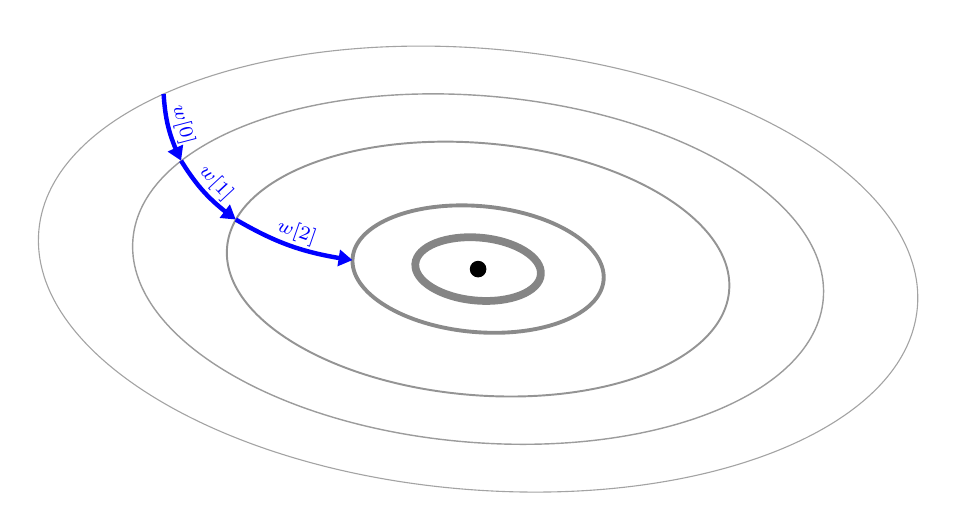
\begin{tikzpicture}[
every edge/.style = {draw, -{Triangle[angle=60:1pt 3,flex]},
                             bend right=11, blue,ultra thick},
every edge quotes/.style = {font=\scriptsize, inner sep=1pt, 
                            auto, sloped}
                            ]
\fill (0,0) circle[radius=3pt];
\path[name path=C] foreach \i in {4, 8, 16, 22, 28}
        {(0,0) circle[draw=red!\i, x radius=2*\i mm, y radius=\i mm, rotate=-5]};
\foreach \i in  {4, 8, 16, 22, 28}
    \draw[line width=11.2/\i, draw=white!\i!gray]
        (0,0) circle[x radius=2*\i mm, y radius=\i mm, rotate=-5];
\path[name path=V] (-4,2.4) .. controls + (0,-2) and + (-2,0) .. (0,0);
%
\draw [name intersections={of=C and V, sort by=C, name=A}]
        (A-5) edge ["${w[0]}$"] (A-4)
        (A-4) edge ["${w[1]}$"] (A-3)
        (A-3) edge ["${w[2]}$"] (A-2);
    \end{tikzpicture}

\part{基于人类反馈的强化学习（RLHF）}

\end{document}